\documentclass{beamer}
% =============================================================================
% ENCODING
% =============================================================================
\usepackage[utf8]{inputenc}  % UTF-8 encoding support

% =============================================================================
% GRAPHICS
% =============================================================================
\usepackage{graphicx}  % For \includegraphics (401 uses across lectures)

% =============================================================================
% MATH PACKAGES
% =============================================================================
\usepackage{amsmath}    % For align, multline, equation environments (heavily used)
\usepackage{amsfonts}   % For \mathbb (e.g., \bbR, \bbE)
\usepackage{amssymb}    % For additional math symbols

% =============================================================================
% TABLES
% =============================================================================
\usepackage{booktabs}   % For \toprule, \midrule, \bottomrule (used in lecture13, lecture14)

% =============================================================================
% LISTS
% =============================================================================
\usepackage{enumerate}  % Enhanced enumerate environment (76 uses across lectures)

% =============================================================================
% TIKZ (DIAGRAMS)
% =============================================================================
\usepackage{tikz}       % For taxonomy diagram and footnotes positioning

% =============================================================================
% UTILITY PACKAGES
% =============================================================================
\usepackage{multido}    % For \multido command used in \eqpause
\usepackage{etoolbox}   % For \AtEndEnvironment, \ifbool, \newbool (used in preamble and taxonomy)
\usepackage{xspace}     % For smart spacing after custom commands (\ODESolve, \SDESolve)

% =============================================================================
% BEAMER THEME SETTINGS
% =============================================================================
\usetheme{default}
\usecolortheme{default}

\setbeamerfont{title}{size=\Huge}
\setbeamertemplate{footline}[frame number]{}
\setbeamertemplate{section in toc}[sections numbered]

\makeatletter
\newcommand\HUGE{\@setfontsize\Huge{35}{40}}
\makeatother    

\setbeamerfont{title}{size=\HUGE}
\beamertemplatenavigationsymbolsempty

% =============================================================================
% TIKZ LIBRARIES
% =============================================================================
% Used for taxonomy diagram: arrows, positioning, shapes
\usetikzlibrary{arrows.meta,calc,shapes,positioning,shadows,trees}

% =============================================================================
% CUSTOM FOOTNOTE COMMANDS
% =============================================================================
% \myfootnote{text} - creates a footnote at the bottom of the slide
\newcommand\myfootnote[1]{%
  \vspace{-0.5cm}%
  \tikz[remember picture,overlay]
  \draw (current page.south west) +(1in + \oddsidemargin,0.5em)
  node[anchor=south west,inner sep=0pt]{\parbox{\textwidth}{%
      \rlap{\rule{10em}{0.4pt}}\raggedright\scriptsize \textit{#1}}};}

% \myfootnotewithlink{url}{text} - creates a clickable footnote (623 uses across lectures)
\newcommand\myfootnotewithlink[2]{%
  \vspace{-0.5cm}%
  \tikz[remember picture,overlay]
  \draw (current page.south west) +(1in + \oddsidemargin,0.5em)
  node[anchor=south west,inner sep=0pt]{\parbox{\textwidth}{%
      \rlap{\rule{10em}{0.4pt}}\raggedright\scriptsize\href{#1}{\textit{#2}}}};}

% =============================================================================
% SECTION/SUBSECTION OUTLINE AUTOMATION
% =============================================================================
% Automatically show outline at the beginning of each section
\AtBeginSection[]
      {
      	\begin{frame}{Outline}
      		\tableofcontents[currentsection]
      	\end{frame}
      }
      \AtBeginSubsection[]{
      	\begin{frame}{Outline}
      		\tableofcontents[currentsection,currentsubsection]
      	\end{frame}
}

% =============================================================================
% CUSTOM SLIDE ANIMATION COMMANDS
% =============================================================================
% These commands enable step-by-step reveal of equations and content
% Used heavily across all lectures (1130+ uses of \nextonslide and \eqpause)

\newcounter{noscounter}   % Counter for \nextonslide (resets on each new slide)
\newcounter{pcounter}     % Counter for pause commands (resets after \eqpause)
\newcounter{diffcounter}  % Counts pauses after equations

% \nextonslide{content} - reveals content on the next overlay
\newcommand{\nextonslide}[1]{%
  \stepcounter{noscounter}%
  \stepcounter{pcounter}%
  \stepcounter{diffcounter}%
  \onslide<\value{noscounter}->{#1}%
}

% \resetonslide - resets all animation counters (called at each frame)
\newcommand{\resetonslide}{%
    \setcounter{noscounter}{1}%
    \setcounter{pcounter}{1}%
    \setcounter{diffcounter}{0}%
}

% \eqpause - pause after equation that syncs with \nextonslide
\newcommand{\eqpause}{%
  \multido{\i=1+1}{\value{pcounter}}{\pause}%
  \stepcounter{noscounter}%
  \setcounter{pcounter}{1}%
}

% \eqpausediff - helper command, runs automatically after math environments
\newcommand{\eqpausediff}{%
  \multido{\i=1+1}{\value{diffcounter}}{\pause}%
  \addtocounter{pcounter}{-\value{diffcounter}}%
  \setcounter{diffcounter}{0}%
}

% Apply \eqpausediff after math environments
\newcommand\AtEndBoth[2]{%
  \AtEndEnvironment{#1}{#2}%
  \AtEndEnvironment{#1*}{#2}%
}

\AtEndBoth{align}{\eqpausediff}
\AtEndBoth{equation}{\eqpausediff}
\AtEndBoth{multline}{\eqpausediff}

% Reset counters at the beginning of each frame
\addtobeamertemplate{frametitle}{\resetonslide}{}

% =============================================================================
% INCLUDE OTHER CONFIGURATION FILES
% =============================================================================
% ==============================================================================
% Custom LaTeX Commands for Deep Generative Models Course
% ==============================================================================

% ==============================================================================
% BOLD LETTERS (mathbf / boldsymbol)
% ==============================================================================

% ------------------------------------------------------------------------------
% Latin Bold Lowercase
% Usage: \bx for x in bold, commonly used for vectors
% ------------------------------------------------------------------------------
\newcommand{\ba}{\mathbf{a}}
\newcommand{\bc}{\mathbf{c}}
\newcommand{\be}{\mathbf{e}}
\newcommand{\bff}{\mathbf{f}}  % Note: \bf is reserved for bold font switching
\newcommand{\bg}{\mathbf{g}}
\newcommand{\bh}{\mathbf{h}}
\newcommand{\bp}{\mathbf{p}}
\newcommand{\bq}{\mathbf{q}}
\newcommand{\bs}{\mathbf{s}}
\newcommand{\bt}{\mathbf{t}}
\newcommand{\bu}{\mathbf{u}}
\newcommand{\bv}{\mathbf{v}}
\newcommand{\bw}{\mathbf{w}}
\newcommand{\bx}{\mathbf{x}}
\newcommand{\by}{\mathbf{y}}
\newcommand{\bz}{\mathbf{z}}
\newcommand{\bzero}{\boldsymbol{0}}  % Zero vector
\newcommand{\bone}{\mathbf{1}}       % Ones vector

% ------------------------------------------------------------------------------
% Latin Bold Uppercase
% Usage: \bX for X in bold, commonly used for matrices or random vectors
% ------------------------------------------------------------------------------
\newcommand{\bA}{\mathbf{A}}
\newcommand{\bG}{\mathbf{G}}
\newcommand{\bI}{\mathbf{I}}
\newcommand{\bJ}{\mathbf{J}}
\newcommand{\bL}{\mathbf{L}}
\newcommand{\bM}{\mathbf{M}}
\newcommand{\bP}{\mathbf{P}}
\newcommand{\bQ}{\mathbf{Q}}
\newcommand{\bR}{\mathbf{R}}
\newcommand{\bT}{\mathbf{T}}
\newcommand{\bU}{\mathbf{U}}
\newcommand{\bV}{\mathbf{V}}
\newcommand{\bW}{\mathbf{W}}
\newcommand{\bX}{\mathbf{X}}
\newcommand{\bZ}{\mathbf{Z}}

% ------------------------------------------------------------------------------
% Greek Bold Lowercase
% Usage: \btheta for θ in bold, commonly used for parameter vectors
% ------------------------------------------------------------------------------
\newcommand{\bepsilon}{\boldsymbol{\epsilon}}
\newcommand{\blambda}{\boldsymbol{\lambda}}
\newcommand{\bmu}{\boldsymbol{\mu}}
\newcommand{\bphi}{\boldsymbol{\phi}}
\newcommand{\bpi}{\boldsymbol{\pi}}
\newcommand{\bpsi}{\boldsymbol{\psi}}
\newcommand{\bsigma}{\boldsymbol{\sigma}}
\newcommand{\btheta}{\boldsymbol{\theta}}

% ------------------------------------------------------------------------------
% Greek Bold Uppercase
% Usage: \bSigma for Σ in bold, commonly used for covariance matrices
% ------------------------------------------------------------------------------
\newcommand{\bPhi}{\boldsymbol{\Phi}}
\newcommand{\bSigma}{\boldsymbol{\Sigma}}
\newcommand{\bTheta}{\boldsymbol{\Theta}}

% ==============================================================================
% CALLIGRAPHIC LETTERS (mathcal)
% Usage: \cX for calligraphic X, commonly used for sets and spaces
% ==============================================================================
\newcommand{\cF}{\mathcal{F}}
\newcommand{\cI}{\mathcal{I}}
\newcommand{\cL}{\mathcal{L}}
\newcommand{\cM}{\mathcal{M}}
\newcommand{\cN}{\mathcal{N}}
\newcommand{\cO}{\mathcal{O}}
\newcommand{\cP}{\mathcal{P}}
\newcommand{\cS}{\mathcal{S}}
\newcommand{\cT}{\mathcal{T}}
\newcommand{\cW}{\mathcal{W}}
\newcommand{\cX}{\mathcal{X}}
\newcommand{\cZ}{\mathcal{Z}}

% ==============================================================================
% BLACKBOARD BOLD LETTERS (mathbb)
% Usage: \bbR for ℝ, commonly used for number sets and expectations
% ==============================================================================
\newcommand{\bbE}{\mathbb{E}}  % Expectation
\newcommand{\bbI}{\mathbb{I}}  % Indicator function
\newcommand{\bbP}{\mathbb{P}}  % Probability measure
\newcommand{\bbR}{\mathbb{R}}  % Real numbers

% ==============================================================================
% MATH OPERATORS
% ==============================================================================

% ------------------------------------------------------------------------------
% Optimization Operators
% Usage: \argmin_{x} f(x) for proper spacing and limits placement
% ------------------------------------------------------------------------------
\DeclareMathOperator*{\argmin}{arg\,min}
\DeclareMathOperator*{\argmax}{arg\,max}

% ------------------------------------------------------------------------------
% Statistical Operators
% Usage: \cov(X, Y) for covariance
% ------------------------------------------------------------------------------
\DeclareMathOperator{\cov}{cov}

% ------------------------------------------------------------------------------
% Linear Algebra Operators
% Usage: \tr(\bA) for trace of matrix A
% ------------------------------------------------------------------------------
\DeclareMathOperator{\tr}{tr}

% ------------------------------------------------------------------------------
% Other Mathematical Operators
% ------------------------------------------------------------------------------
\DeclareMathOperator{\diver}{div}      % Divergence (vector calculus)
\newcommand{\sg}{\mathrm{sg}}          % Stop-gradient operator
\DeclareMathOperator{\softmax}{softmax}
\DeclareMathOperator{\supp}{supp}      % Support of a distribution

% ==============================================================================
% PROBABILITY DISTRIBUTIONS
% Usage: X \sim \cN(0, 1), Y \sim \Bern(p)
% ==============================================================================
\DeclareMathOperator{\Bern}{Bern}      % Bernoulli distribution
\DeclareMathOperator{\Cat}{Cat}        % Categorical distribution
\DeclareMathOperator{\Gumbel}{Gumbel}  % Gumbel distribution
\DeclareMathOperator{\Uniform}{Uniform}

% ==============================================================================
% METRICS AND DIVERGENCES
% Usage: \KL(p \| q), \JSD(p, q)
% ==============================================================================
\newcommand{\Ent}{\mathrm{H}}          % Entropy
\newcommand{\FID}{\mathrm{FID}}        % Fréchet Inception Distance
\newcommand{\JSD}{D_\mathrm{JS}}        % Jensen-Shannon Divergence
\newcommand{\KL}{D_\mathrm{KL}}        % Kullback-Leibler Divergence
\DeclareMathOperator{\MMD}{MMD}        % Maximum Mean Discrepancy
\DeclareMathOperator{\SNR}{SNR}        % Signal-to-Noise Ratio

% ==============================================================================
% NEURAL NETWORK NOTATION
% ==============================================================================

% ------------------------------------------------------------------------------
% Network Architectures (upright font for abbreviations)
% Usage: f_{\btheta} = \NN_{\btheta}(\bx)
% ------------------------------------------------------------------------------
\newcommand{\MLP}{\mathrm{MLP}}        % Multi-Layer Perceptron
\newcommand{\NN}{\mathrm{NN}}          % Neural Network
\newcommand{\RNN}{\mathrm{RNN}}        % Recurrent Neural Network

% ------------------------------------------------------------------------------
% Numerical Solvers (monospace font)
% Usage: \bx_T = \ODESolve(v, \bx_0, T)
% ------------------------------------------------------------------------------
\newcommand{\ODESolve}{\texttt{ODESolve}\xspace}
\newcommand{\SDESolve}{\texttt{SDESolve}\xspace}

% ==============================================================================
% COMMON SHORTCUTS
% Usage: Frequently used subscripted or parameterized expressions
% ==============================================================================
\newcommand{\pd}{p_{\text{data}}}              % Data distribution
\newcommand{\pt}{p_{\boldsymbol{\theta}}}      % Parameterized distribution
\newcommand{\qagg}{q_{\text{agg}}}             % Aggregated posterior
\newcommand{\lambdamax}{\lambda_{\text{max}}}  % Maximum eigenvalue
  % Math shorthand commands (\bx, \bbE, \KL, etc.)
\input{../utils/title}        % Title page template
% For each possible node, we create a boolean
\newbool{hl@root}
\newbool{hl@explicit}
\newbool{hl@implicit}
\newbool{hl@exact}
\newbool{hl@approx}
\newbool{hl@gan}
\newbool{hl@ar}
\newbool{hl@nf}
\newbool{hl@vae}
\newbool{hl@score}
\newbool{hl@cont}
\newbool{hl@ddpm}
\newbool{hl@sm}
\newbool{hl@ode}
\newbool{hl@sde}
\newbool{hl@fm}

% Command to reset all bools
\newcommand{\resetAllHighlights}{%
    \boolfalse{hl@root}%
    \boolfalse{hl@explicit}%
    \boolfalse{hl@implicit}%
    \boolfalse{hl@exact}%
    \boolfalse{hl@approx}%
    \boolfalse{hl@gan}%
    \boolfalse{hl@ar}%
    \boolfalse{hl@nf}%
    \boolfalse{hl@vae}%
    \boolfalse{hl@score}%
    \boolfalse{hl@cont}%
    \boolfalse{hl@ddpm}%
    \boolfalse{hl@sm}%
    \boolfalse{hl@ode}%
    \boolfalse{hl@sde}%
    \boolfalse{hl@fm}%
}

% Command to set a single highlight
\newcommand{\setHighlight}[1]{%
    \booltrue{hl@#1}%
}

% Command to set highlights from comma-separated list
\newcommand{\setHighlights}[1]{%
    \resetAllHighlights%
    \forcsvlist{\setHighlight}{#1}%
}

% Highlighted style definition
\tikzset{
    hl/.style={line width=1.2pt, draw=black, font=\scriptsize\bfseries},
    box/.style={
        rectangle, 
        draw=gray!50, 
        rounded corners=2pt, 
        minimum width=1.9cm, 
        minimum height=0.5cm, 
        align=center, 
        font=\scriptsize, 
        line width=0.4pt
    },
    rootnode/.style={box, fill=violet!20},
    category/.style={box, fill=teal!20},
    model/.style={box, fill=yellow!30},
    arrow/.style={-Stealth, draw=gray!80, line width=0.4pt}
}

% Draw taxonomy with pre-set highlights
\newcommand{\drawTaxonomy}{%
    \begin{tikzpicture}[scale=0.9, transform shape, node distance=0.6cm and 0.3cm]
        % --- CENTRAL ROOT ---
        \ifbool{hl@root}{\node[rootnode, hl] (root) {Generative Models};}{\node[rootnode] (root) {Generative Models};}

        % --- UPPER BRANCHES ---
        \ifbool{hl@explicit}{\node[category, hl, above left=0.6cm and 0.5cm of root] (explicit) {Explicit density};}{\node[category, above left=0.6cm and 0.5cm of root] (explicit) {Explicit density};}
        \ifbool{hl@implicit}{\node[category, hl, above right=0.6cm and 0.5cm of root] (implicit) {Implicit density};}{\node[category, above right=0.6cm and 0.5cm of root] (implicit) {Implicit density};}

        \ifbool{hl@exact}{\node[category, hl, above left=0.6cm and -0.6cm of explicit] (exact) {Exact likelihood};}{\node[category, above left=0.6cm and -0.6cm of explicit] (exact) {Exact likelihood};}
        \ifbool{hl@approx}{\node[category, hl, above right=0.6cm and -0.6cm of explicit] (approx) {Approximate likelihood};}{\node[category, above right=0.6cm and -0.6cm of explicit] (approx) {Approximate likelihood};}

        \ifbool{hl@gan}{\node[model, hl, above=0.6cm of implicit] (gans) {GANs};}{\node[model, above=0.6cm of implicit] (gans) {GANs};}

        \ifbool{hl@ar}{\node[model, hl, above left=0.6cm and -0.9cm of exact] (ar) {Autoregressive \\ models};}{\node[model, above left=0.6cm and -0.9cm of exact] (ar) {Autoregressive \\ models};}
        \ifbool{hl@nf}{\node[model, hl, above right=0.6cm and -0.9cm of exact] (nf) {Normalizing \\ Flows};}{\node[model, above right=0.6cm and -0.9cm of exact] (nf) {Normalizing \\ Flows};}
        \ifbool{hl@vae}{\node[model, hl, above=0.6cm of approx] (vae) {Variational \\ Autoencoders};}{\node[model, above=0.6cm of approx] (vae) {Variational \\ Autoencoders};}

        % --- LOWER BRANCHES ---
        \ifbool{hl@score}{\node[category, hl, below left=0.6cm and 0.5cm of root] (score) {Score-based};}{\node[category, below left=0.6cm and 0.5cm of root] (score) {Score-based};}
        \ifbool{hl@cont}{\node[category, hl, below right=0.6cm and 0.5cm of root] (cont) {Continuous \\ dynamics};}{\node[category, below right=0.6cm and 0.5cm of root] (cont) {Continuous \\ dynamics};}

        \ifbool{hl@sm}{\node[model, hl, below left=0.6cm and -0.8cm of score] (sm) {Score Matching};}{\node[model, below left=0.6cm and -0.8cm of score] (sm) {Score Matching};}
        \ifbool{hl@ddpm}{\node[model, hl, below right=0.6cm and -0.8cm of score] (ddpm) {Denoising Diffusion};}{\node[model, below right=0.6cm and -0.8cm of score] (ddpm) {Denoising Diffusion};}

        \ifbool{hl@ode}{\node[model, hl, below left=0.6cm and -0.8cm of cont] (ode) {Neural ODEs};}{\node[model, below left=0.6cm and -0.8cm of cont] (ode) {Neural ODEs};}
        \ifbool{hl@sde}{\node[model, hl, below right=0.6cm and -0.8cm of cont] (sde) {SDE-based \\ Diffusion};}{\node[model, below right=0.6cm and -0.8cm of cont] (sde) {SDE-based \\ Diffusion};}

        \ifbool{hl@fm}{\node[model, hl, below=0.6cm of ode] (fm) {Flow Matching};}{\node[model, below=0.6cm of ode] (fm) {Flow Matching};}

        % --- CONNECTIONS ---
        \draw[arrow] (root.north) -- ++(0,0.3) -| (explicit.south);
        \draw[arrow] (root.north) -- ++(0,0.3) -| (implicit.south);
        \draw[arrow] (root.south) -- ++(0,-0.3) -| (score.north);
        \draw[arrow] (root.south) -- ++(0,-0.3) -| (cont.north);
        \draw[arrow] (explicit.north) -- ++(0,0.3) -| (exact.south);
        \draw[arrow] (explicit.north) -- ++(0,0.3) -| (approx.south);
        \draw[arrow] (exact.north) -- ++(0,0.3) -| (ar.south);
        \draw[arrow] (exact.north) -- ++(0,0.3) -| (nf.south);
        \draw[arrow] (approx.north) -- (vae.south);
        \draw[arrow] (implicit.north) -- (gans.south);
        \draw[arrow] (score.south) -- ++(0,-0.3) -| (sm.north);
        \draw[arrow] (score.south) -- ++(0,-0.3) -| (ddpm.north);
        \draw[arrow] (cont.south) -- ++(0,-0.3) -| (ode.north);
        \draw[arrow] (cont.south) -- ++(0,-0.3) -| (sde.north);
        \draw[arrow] (ode.south) -- (fm.north);
    \end{tikzpicture}
}

% The main taxonomy rendering command
\newcommand{\renderTaxonomy}[1]{%
    \setHighlights{#1}%
    \centering
    \drawTaxonomy%
}     % Generative models taxonomy diagram

\createdgmtitle{6}
%--------------------------------------------------------------------------------
\begin{document}
%--------------------------------------------------------------------------------
\begin{frame}[noframenumbering,plain]
	\titlepage
	\resetonslide
\end{frame}
%=======
\begin{frame}{Recap of Previous Lecture}
	\myfootnotewithlink{https://arxiv.org/abs/1406.2661}{Goodfellow I. J. et al. Generative Adversarial Networks, 2014}
	\begin{block}{GAN Optimality Theorem}
		The minimax game
		\[
		\min_{G} \max_D \Bigl[ \underbrace{\bbE_{\pd(\bx)} \log D(\bx) + \bbE_{p(\bz)} \log (1 - D(\bG(\bz)))}_{V(G, D)} \Bigr]
		\]
		has a global optimum at $\pd(\bx) = \pt(\bx)$, and then $D^*(\bx) = 0.5$.
	\end{block}
	\vspace{-0.3cm}
	\[
		\min_{G} V(G, D^*) = \min_{G} \left[ 2 \JSD(\pi \| p) - \log 4 \right] = -\log 4, \quad \pd(\bx) = \pt(\bx).
	\]
	If the generator can be \textbf{any} function and the discriminator is \textbf{optimal} at each step, then the generator is \textbf{guaranteed to converge} to the data distribution.  
\end{frame}
%=======
\begin{frame}{Recap of Previous Lecture}
	\myfootnotewithlink{https://arxiv.org/abs/1406.2661}{Goodfellow I. J. et al. Generative Adversarial Networks, 2014}
	\begin{itemize}
		\item The generator is updated in the parameter space; the discriminator isn't optimal at every iteration.
		\item Both generator and discriminator loss typically oscillate during GAN training.
	\end{itemize}
	\begin{block}{Objective}
		\vspace{-0.5cm}
		\[
		\min_{\btheta} \max_{\bphi} \left[ \bbE_{\pd(\bx)} \log D_{\bphi}(\bx) + \bbE_{p(\bz)} \log (1 - D_{\bphi}(\bG_{\btheta}(\bz))) \right]
		\]
		\vspace{-0.5cm}
	\end{block}
	\begin{figure}
		\centering
		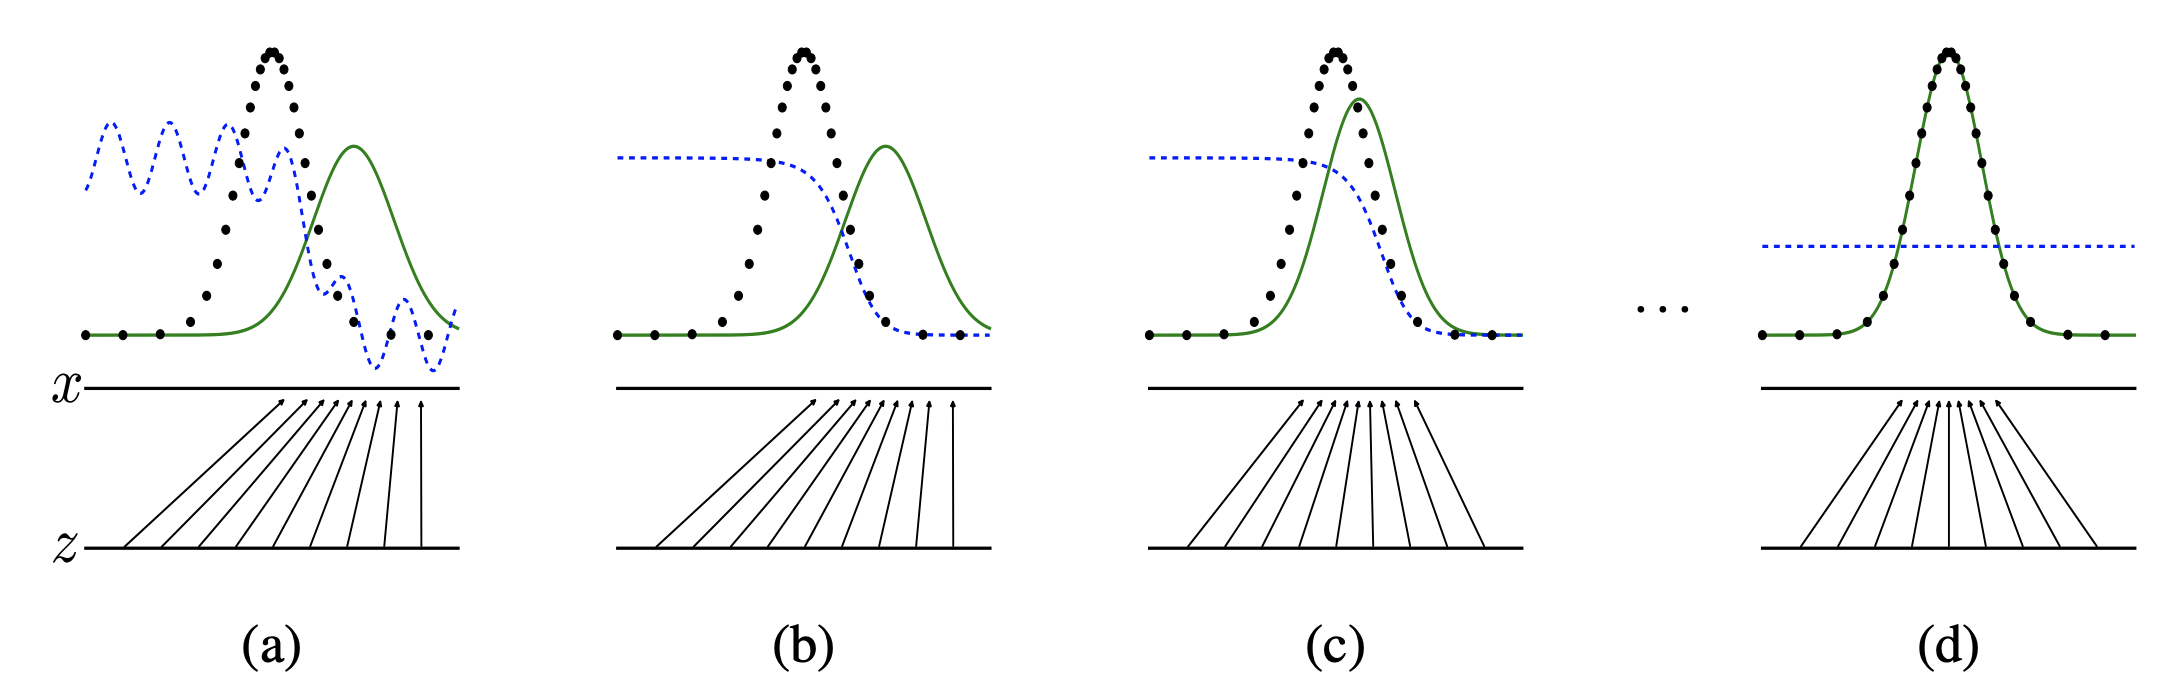
\includegraphics[width=1.0\linewidth]{figs/gan_1}
	\end{figure}
\end{frame}
%=======
\begin{frame}{Recap of Previous Lecture}
	\myfootnote{\href{https://arxiv.org/abs/1406.2661}{Goodfellow I. J. et al. Generative Adversarial Networks, 2014} \\
		\href{https://arxiv.org/abs/1701.04862}{Arjovsky M., Bottou L. Towards Principled Methods for Training Generative Adversarial Networks, 2017}}
	\begin{block}{Main Issues With Standard GANs}
		\begin{itemize}
			\item Vanishing gradients (solution: non-saturating GAN).
			\item Mode collapse (arises from Jensen-Shannon divergence).
		\end{itemize}
	\end{block}
	\begin{block}{Standard GAN}
		\vspace{-0.2cm}
		\[
		\min_{\btheta} \max_{\bphi} \left[ \bbE_{\pd(\bx)} \log D_{\bphi}(\bx) + \bbE_{p(\bz)} \log (1 - D_{\bphi}(\bG_{\btheta}(\bz))) \right]
		\]
		\vspace{-0.4cm}
	\end{block}
	\vspace{-0.1cm}
	\begin{block}{Informal Theoretical Results}
		Both the data distribution $\pd(\bx)$ and the generative distribution $\pt(\bx)$ are low-dimensional with disjoint supports. In such cases,
		\[
			\KL(\pd \| \pt) = \KL(\pt \| \pd) = \infty, \quad \JSD(\pd \| \pt) = \log 2.
		\]
	\end{block}
\end{frame}
%=======
\begin{frame}{Recap of Previous Lecture}
	\myfootnotewithlink{https://udlbook.github.io/udlbook/}{Simon J.D. Prince. Understanding Deep Learning, 2023}
	\begin{figure}
		\centering
		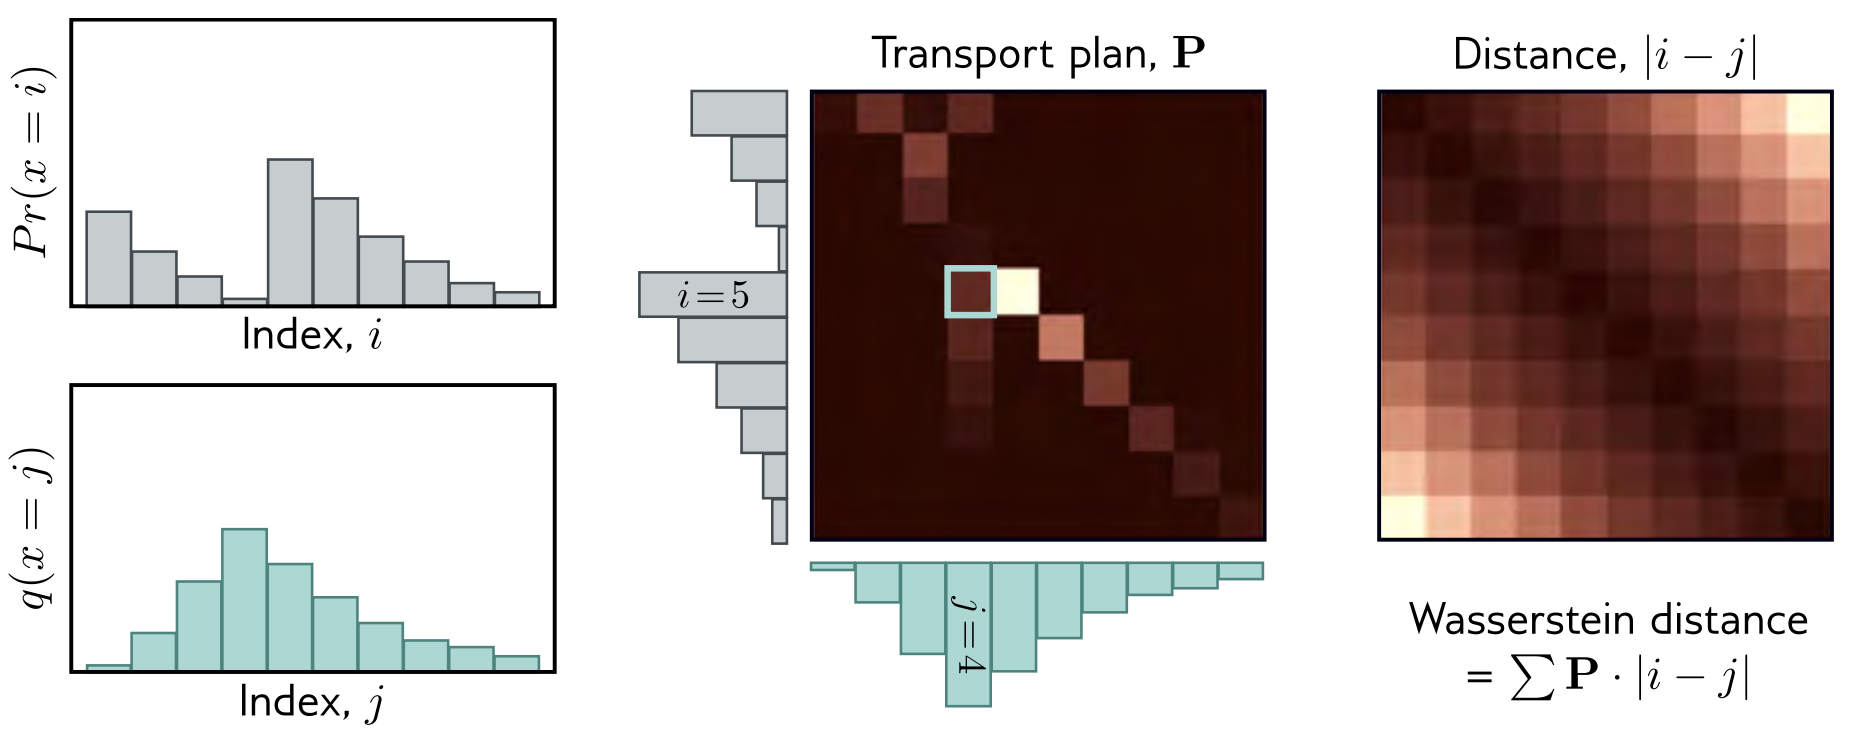
\includegraphics[width=0.8\linewidth]{figs/discrete_wasserstein}
	\end{figure}
	\vspace{-0.3cm}
	\begin{block}{Wasserstein Distance}
		\vspace{-0.7cm}
		{\small
		\[
		W(\pi \| p) = \inf_{\gamma \in \Gamma(\pi, p)} \bbE_{(\bx_1, \bx_2) \sim \gamma} \| \bx_1 - \bx_2 \| =  \inf_{\gamma \in \Gamma(\pi, p)} \int \| \bx_1 - \bx_2 \| \gamma (\bx_1, \bx_2) d \bx_1 d \bx_2
		\]
		}
		\vspace{-0.5cm}
		\begin{itemize}
			\item $\gamma(\bx_1, \bx_2)$ -- transportation plan (amount of "dirt" to transport from $\bx_1$ to $\bx_2$).
			\item $\Gamma(\pi, p)$ -- set of all joint distributions $\gamma (\bx_1, \bx_2)$ with marginals $\pi$ and $p$ ($\int \gamma(\bx_1, \bx_2) d \bx_1 = p(\bx_2)$, $\int \gamma(\bx_1, \bx_2) d \bx_2 = \pi(\bx_1)$).
			\item $\gamma(\bx_1, \bx_2)$ -- the amount; $\|\bx_1 - \bx_2 \|$ -- the distance.
		\end{itemize}
	\end{block}
\end{frame}
%=======
\begin{frame}{Recap of Previous Lecture}
	\myfootnotewithlink{https://arxiv.org/abs/1701.07875}{Arjovsky M., Chintala S., Bottou L. Wasserstein GAN, 2017}
	\begin{block}{Theorem (Kantorovich-Rubinstein Duality)}
		\vspace{-0.2cm}
		\[
		W(\pd \| \pt) = \frac{1}{K} \max_{\| f \|_L \leq K} \left[ \bbE_{\pd(\bx)} f(\bx)  - \bbE_{\pt(\bx)} f(\bx)\right],
		\]
		where $\| f \|_L \leq K$ denotes $K$-Lipschitz continuous functions.
	\end{block}
	\begin{block}{WGAN Objective}
		\vspace{-0.5cm}
		\[
		\min_{\btheta} {\color{violet}W(\pd \| \pt)} = \min_{\btheta} {\color{violet}\max_{\bphi \in \boldsymbol{\Phi}} \left[ \bbE_{\pd(\bx)} f_{\bphi}(\bx)  - \bbE_{p(\bz)} f_{\bphi}(\bG_{\btheta}(\bz))\right]}.
		\]
		\vspace{-0.5cm}
	\end{block}
	\begin{itemize}
		\item The function $f$ in WGAN is called the \textit{critic}.
		\item If parameters $\bphi$ lie in a compact set $\boldsymbol{\Phi} \in [-c, c]^d$, then $f(\bx, \bphi)$ is $K$-Lipschitz continuous. 
	\end{itemize}
	\begin{multline*}
		K \cdot W(\pd \| \pt) = \max_{\| f \|_L \leq K} \left[ \bbE_{\pd(\bx)} f(\bx) - \bbE_{\pt(\bx)} f(\bx)\right] \geq 
		\\ \geq \max_{\bphi \in \boldsymbol{\Phi}} \left[ \bbE_{\pd(\bx)} f_{\bphi}(\bx)  - \bbE_{\pt(\bx)} f_{\bphi}(\bx)\right]
	\end{multline*}
\end{frame}
%=======
\begin{frame}{Recap of Previous Lecture}
    \myfootnotewithlink{https://arxiv.org/abs/1706.08500}{Heusel M. et al. GANs Trained by a Two Time-Scale Update Rule Converge to a Local Nash Equilibrium, 2017}
	\vspace{-0.3cm}
	\begin{block}{Frechet Inception Distance (FID)}
		For normal distributions $\pd(\bx_1) = \cN(\bmu_{\text{data}}, \bSigma_{\text{data}})$, $p(\bx_2) = \cN(\bmu_{\boldsymbol{\theta}}, \bSigma_{\boldsymbol{\theta}})$:
		\vspace{-0.3cm}
		\begin{multline*}
			\FID (\pd, \pt) =  W_2^2(\pd, \pt) = \inf_{\gamma \in \Gamma(\pd, \pt)} \bbE_{(\bx_1, \bx_2) \sim \gamma} \| \bx_1 - \bx_2 \|^2 \\
			= \| \bmu_{\text{data}} - \bmu_{\boldsymbol{\theta}}\|^2 + \tr \left[ \bSigma_{\text{data}} + \bSigma_{\boldsymbol{\theta}} - 2 \left(\bSigma_{\text{data}}^{1/2} \bSigma_{\boldsymbol{\theta}} \bSigma_{\text{data}}^{1/2} \right)^{1/2} \right]
		\end{multline*}
		\vspace{-0.4cm}
	\end{block}
	\begin{itemize}
		\item Requires a large sample size for evaluation
		\item FID computation is relatively slow
		\item Results are highly dependent on the chosen pretrained classifier
		\item Relies on the normality assumption
	\end{itemize}
\end{frame}
%=======
\begin{frame}{Recap of Previous Lecture}
    \myfootnotewithlink{https://arxiv.org/abs/1904.06991}{Kynkäänniemi T. et al. Improved precision and recall metric for assessing generative models, 2019}
	\vspace{-0.3cm}
	\begin{itemize}
		\item $\cS_{\text{data}} = \{\bx_i\}_{i=1}^{n} \sim \pd(\bx)$: real samples
		\item $\cS_{\btheta} = \{\bx_i\}_{i=1}^{n} \sim \pt(\bx)$: generated samples
	\end{itemize}
	Define a binary indicator function:
	\vspace{-0.2cm}
	\[
		\bbI(\bx, \cS) = 
		\begin{cases}
			1, & \text{if}~ \exists~ \bx' \in \cS: \| \bx  - \bx'\|_2 \leq \| \bx' - \NN_k(\bx', \cS)\|_2; \\
			0, & \text{otherwise}
		\end{cases}
	\]
	\vspace{-0.3cm}
	\[
		\text{Pr} (\cS_{\text{data}}, \cS_{\btheta}) = \frac{1}{n} \sum_{\bx \in \cS_{\btheta}} \bbI(\bx, \cS_{\text{data}}); \quad \text{Rec} (\cS_{\text{data}}, \cS_{\btheta}) = \frac{1}{n} \sum_{\bx \in \cS_{\text{data}}} \bbI(\bx, \cS_{\btheta}).
	\]
	\vspace{-0.5cm}
	\begin{figure}
		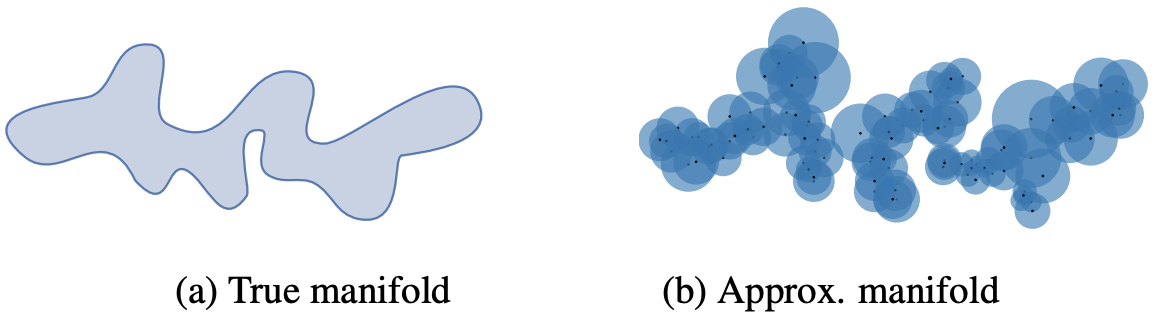
\includegraphics[width=0.75\linewidth]{figs/pr_k_nearest}
	\end{figure}
	\vspace{-0.3cm}
	The samples are embedded using a pretrained network, as in FID evaluation.
\end{frame}
%=======
\begin{frame}{Recap of Previous Lecture}
    \myfootnotewithlink{https://arxiv.org/abs/2103.00020}{Radford A. et al. Learning transferable visual models from natural language supervision, 2021} 
	\vspace{-0.2cm}
	\begin{minipage}{0.5\linewidth}
		\begin{block}{Unconditional Model}
			\begin{figure}
				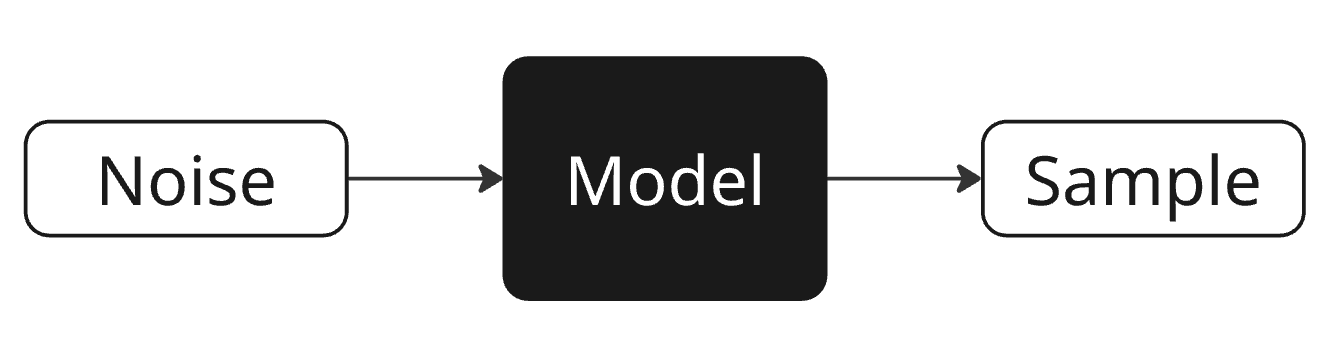
\includegraphics[width=0.95\linewidth]{figs/uncond_model}
			\end{figure}
		\end{block}
	\end{minipage}%
	\begin{minipage}{0.5\linewidth}
		\vspace{0.2cm}
		\begin{block}{Conditional Model}
			\begin{figure}
				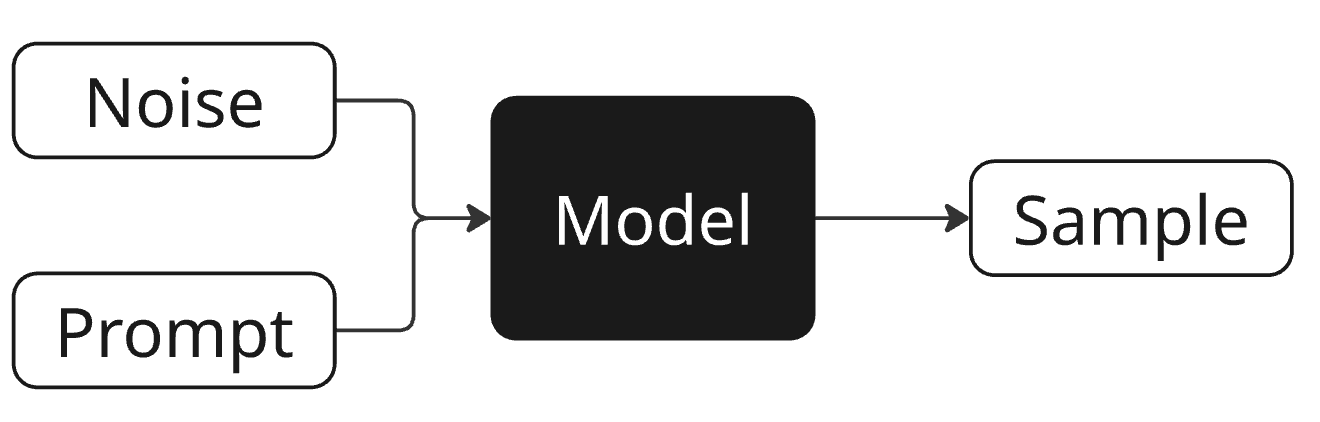
\includegraphics[width=0.95\linewidth]{figs/cond_model}
			\end{figure}
		\end{block}
	\end{minipage}
	We require metrics that evaluate not only the quality of generated images, but also their relevance to the prompt.
	\begin{block}{CLIP Score}
		\begin{figure}
			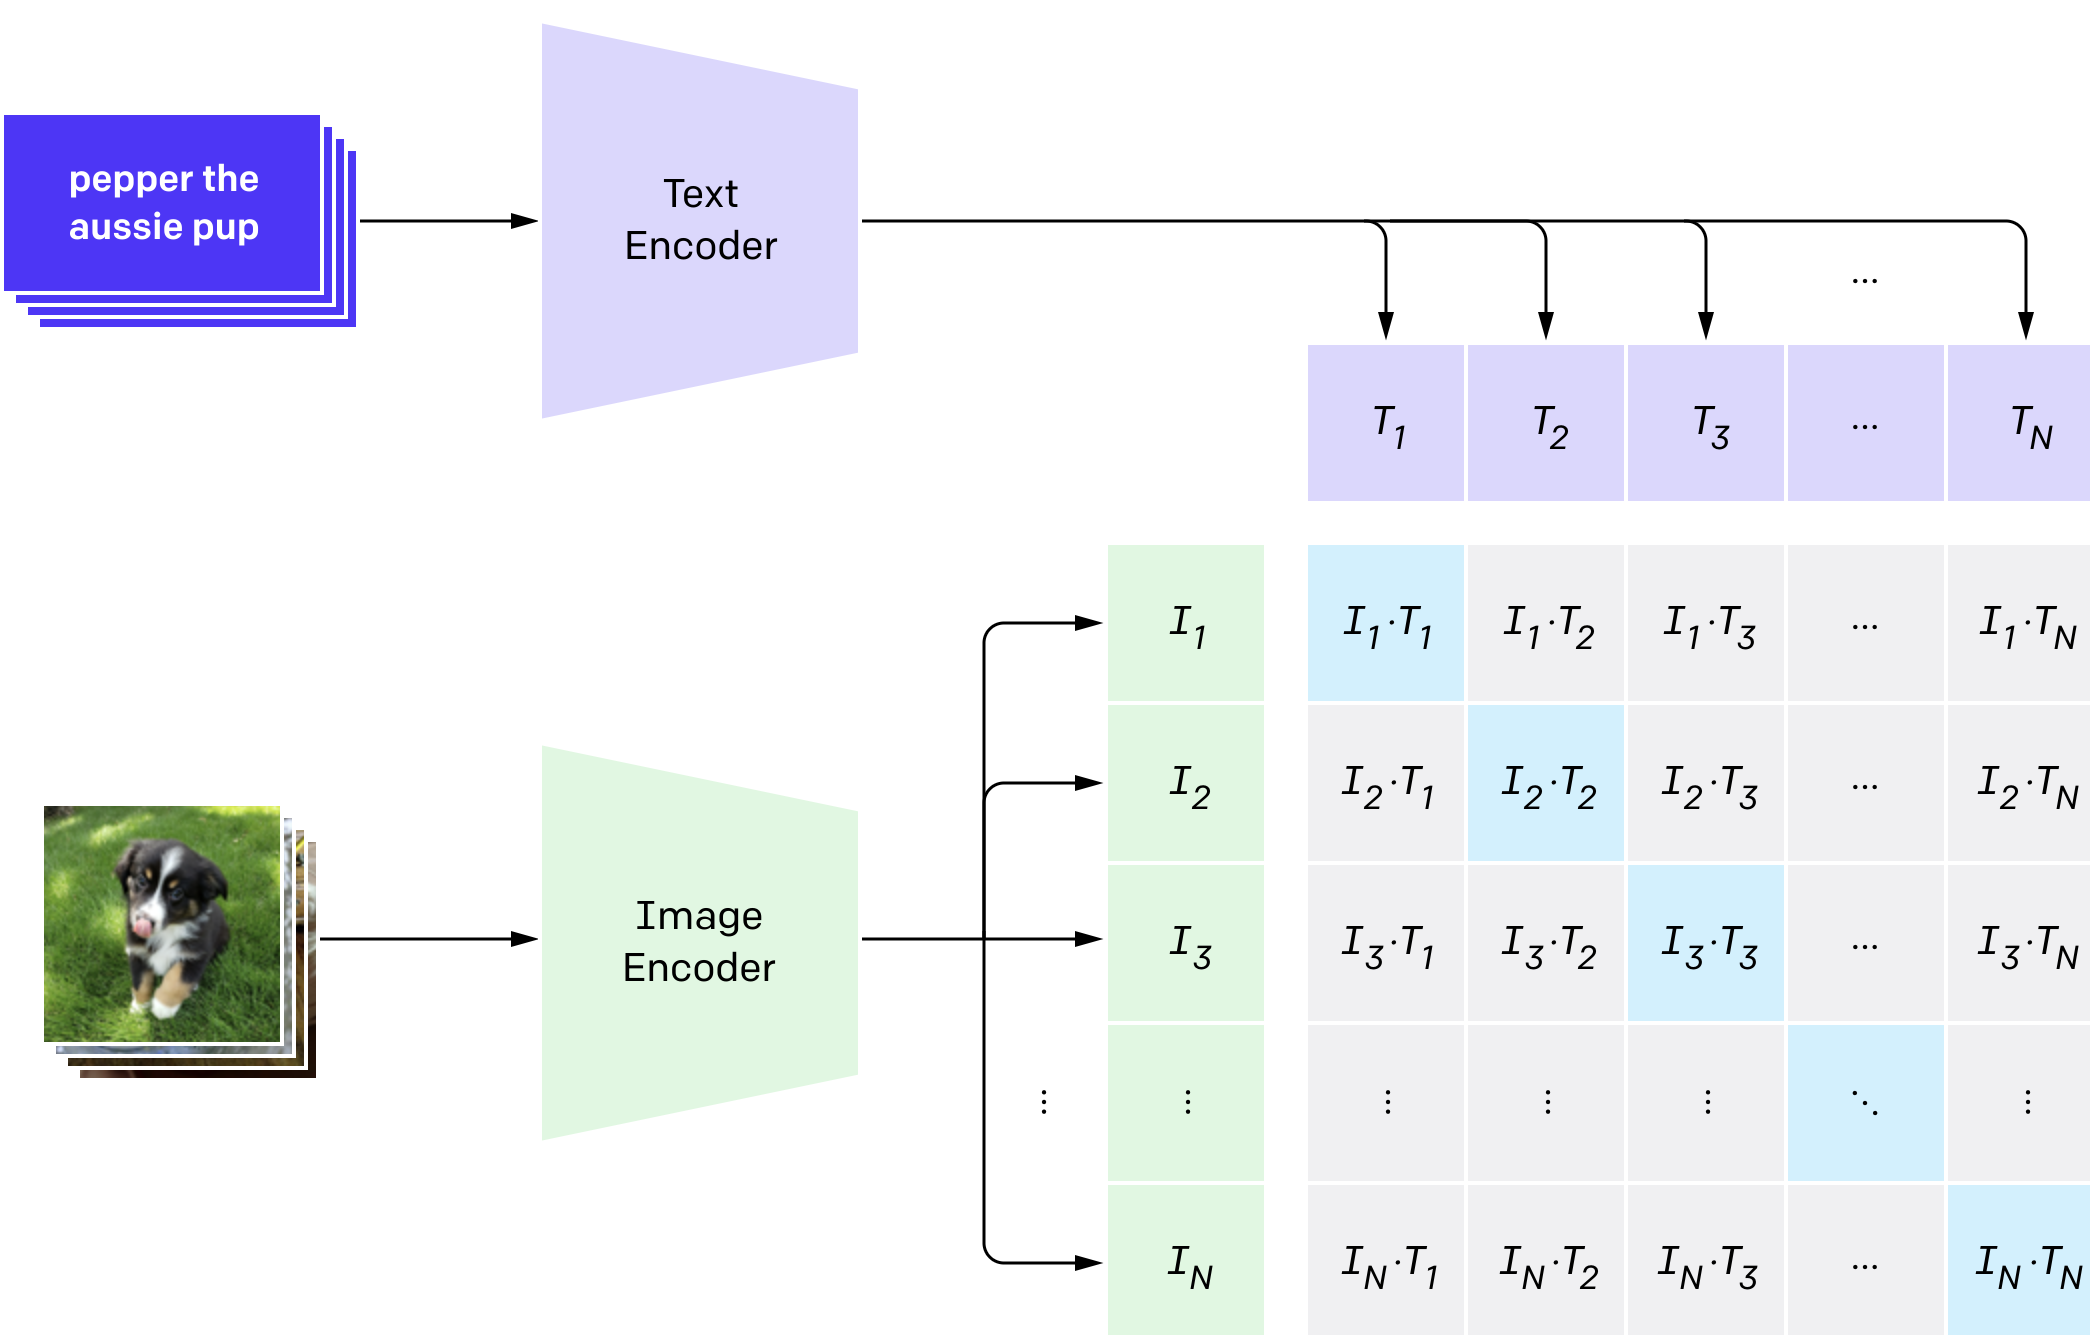
\includegraphics[width=0.5\linewidth]{figs/clip}
		\end{figure}
	\end{block}
\end{frame}
%=======
\begin{frame}{Recap of Previous Lecture}
    \myfootnotewithlink{https://ya.ru/ai/art}{YandexART 2.5, 2025} 
	\begin{itemize}
		\item No perfect automatic evaluation metric exists
		\item The most reliable assessment is via human evaluation
		\item It's important to evaluate a variety of model aspects
	\end{itemize}
	\begin{block}{Human Evaluation}
		\begin{figure}
			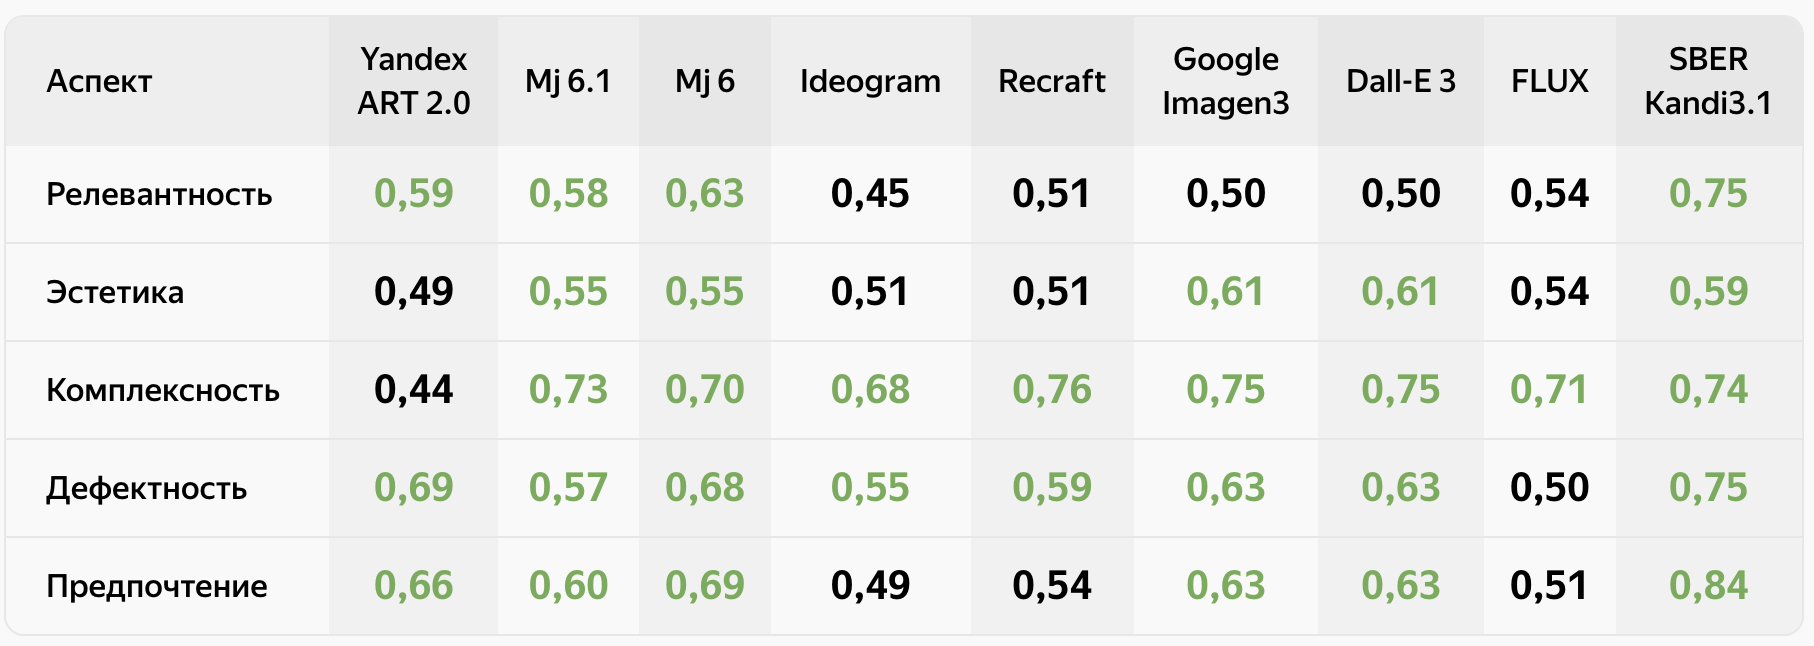
\includegraphics[width=1.0\linewidth]{figs/yaart_2.5}
		\end{figure}
	\end{block}
\end{frame}
%=======
\begin{frame}{Outline}
	\tableofcontents
\end{frame}
%=======
\section{Langevin Dynamics}
%=======
\begin{frame}{Energy-Based Models}
	\begin{block}{Unnormalized Density}
		\vspace{-0.2cm}
		\[
			\pt(\bx) = \frac{\hat{p}_{\btheta}(\bx)}{Z_{\btheta}}, \quad \text{where } Z_{\btheta} = \int \hat{p}_{\btheta}(\bx) d \bx
		\]
		\vspace{-0.3cm}
		\begin{itemize}
			\item $\hat{p}_{\btheta}(\bx)$ can be any non-negative function. \\
			\item If we reparameterize as $\hat{p}_{\btheta}(\bx) = \exp(-f_{\btheta}(\bx))$, we eliminate the non-negativity constraint.
		\end{itemize}
	\end{block}
	\eqpause
	\vspace{-0.3cm}
	\begin{block}{Unnormalized Density}
		The gradient of the normalized log-density equals that of the unnormalized log-density:
		\[
			\nabla_{\bx} \log \pt(\bx) = \nabla_{\bx} \log \hat{p}_{\btheta}(\bx) - \nabla_{\bx} \log Z_{\btheta} = \nabla_{\bx} \log \hat{p}_{\btheta}(\bx)
		\]
	\end{block}
	\eqpause
	\vspace{-0.3cm}
	\begin{itemize}
		\item Suppose we already have this density (normalized or not) $\pt(\bx)$.
		\item How can we sample from the model?
	\end{itemize}
\end{frame}
%=======
\begin{frame}{Langevin Dynamics}
	\myfootnotewithlink{https://arxiv.org/abs/2510.21890}{Lai C. H. et al. The principles of diffusion models, 2025.}
	\vspace{-0.4cm}
	\begin{block}{Theorem (Informal)}
		Let $\bx_0$ be a random vector. Under mild regularity conditions, samples from the following dynamics will eventually follow $\pt(\bx)$ (for sufficiently small $\eta$ and large $l$):
		\vspace{-0.3cm}
		\[
			\bx_{l + 1} = \bx_l + \frac{\eta}{2} \cdot \nabla_{\bx_l} \log \pt(\bx_l) + \sqrt{\eta} \cdot \bepsilon_l, \quad \bepsilon_l \sim \cN(0, \bI).
		\]
		\vspace{-0.5cm}
	\end{block}
	\eqpause
	\begin{minipage}{0.55\linewidth}
		\begin{itemize}
			\item What if $\bepsilon_l = \boldsymbol{0}$?
			\item The density $\pt(\bx)$ is the \textbf{stationary} distribution of the Markov chain.
			\item The gradient is taken with respect to $\bx$, not $\btheta$.
			\item $\nabla_{\bx} \log \pt(\bx)$ defines a vector field.
		\end{itemize}
	\end{minipage}%
	\begin{minipage}{0.45\linewidth}
		\begin{figure}
			\centering
			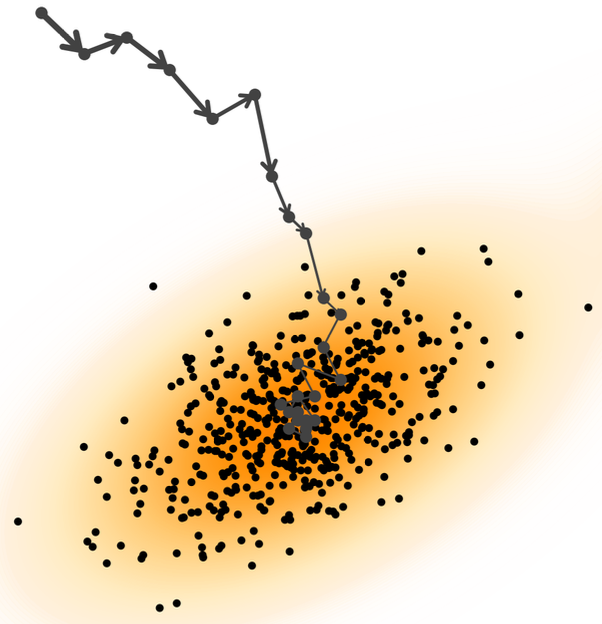
\includegraphics[width=0.9\linewidth]{figs/langevin_dynamic}
		\end{figure}
	\end{minipage}
\end{frame}
%=======
\section{Score Matching}
%=======
\begin{frame}{Generative Models Taxonomy}
	\renderTaxonomy{sm}
\end{frame}
%=======
\begin{frame}{Score Function}
	\myfootnotewithlink{https://arxiv.org/abs/2510.21890}{Lai C. H. et al. The principles of diffusion models, 2025.}
	\vspace{-0.3cm}
	\[
		\bs_{\btheta}(\bx) = \nabla_{\bx}\log \pt(\bx)
	\]
	\vspace{-0.5cm}
	\begin{figure}
		\centering
		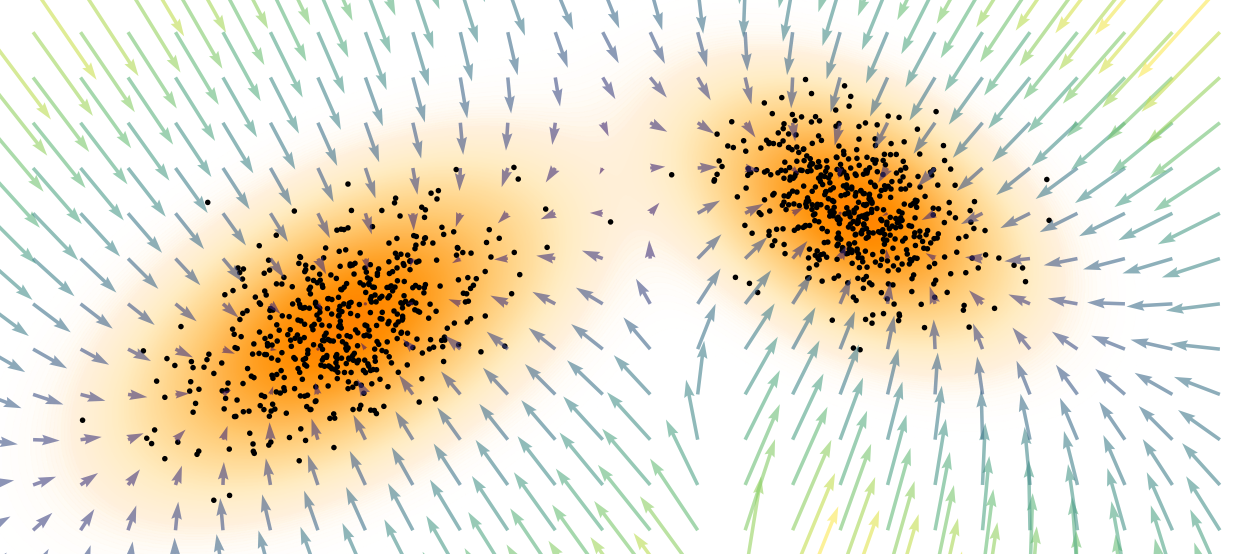
\includegraphics[width=0.8\linewidth]{figs/score_function}
	\end{figure}
	\vspace{-0.3cm}
	\eqpause
	\begin{block}{Langevin Dynamics}
		\vspace{-0.5cm}
		\begin{multline*}
			\bx_{l + 1} = \bx_l + \frac{\eta}{2} \cdot \nabla_{\bx_l} \log \pd(\bx_l) + \sqrt{\eta} \cdot \bepsilon_l \\
			= \bx_l + \frac{\eta}{2} \cdot {\color{violet}\nabla_{\bx_l} \log \pt(\bx_l)} + \sqrt{\eta} \cdot \bepsilon_l 
			= \bx_l + \frac{\eta}{2} \cdot {\color{violet}\bs_{\btheta}(\bx_l)} + \sqrt{\eta} \cdot \bepsilon_l.
		\end{multline*}
		\vspace{-0.5cm}
	\end{block}
\end{frame}
%=======
\begin{frame}{Score Matching}
	\myfootnotewithlink{https://yang-song.github.io/blog/2021/score/}{Song Y. Generative Modeling by Estimating Gradients of the Data Distribution, blog post, 2021}
	\vspace{-0.5cm}
	\begin{figure}
		\centering
		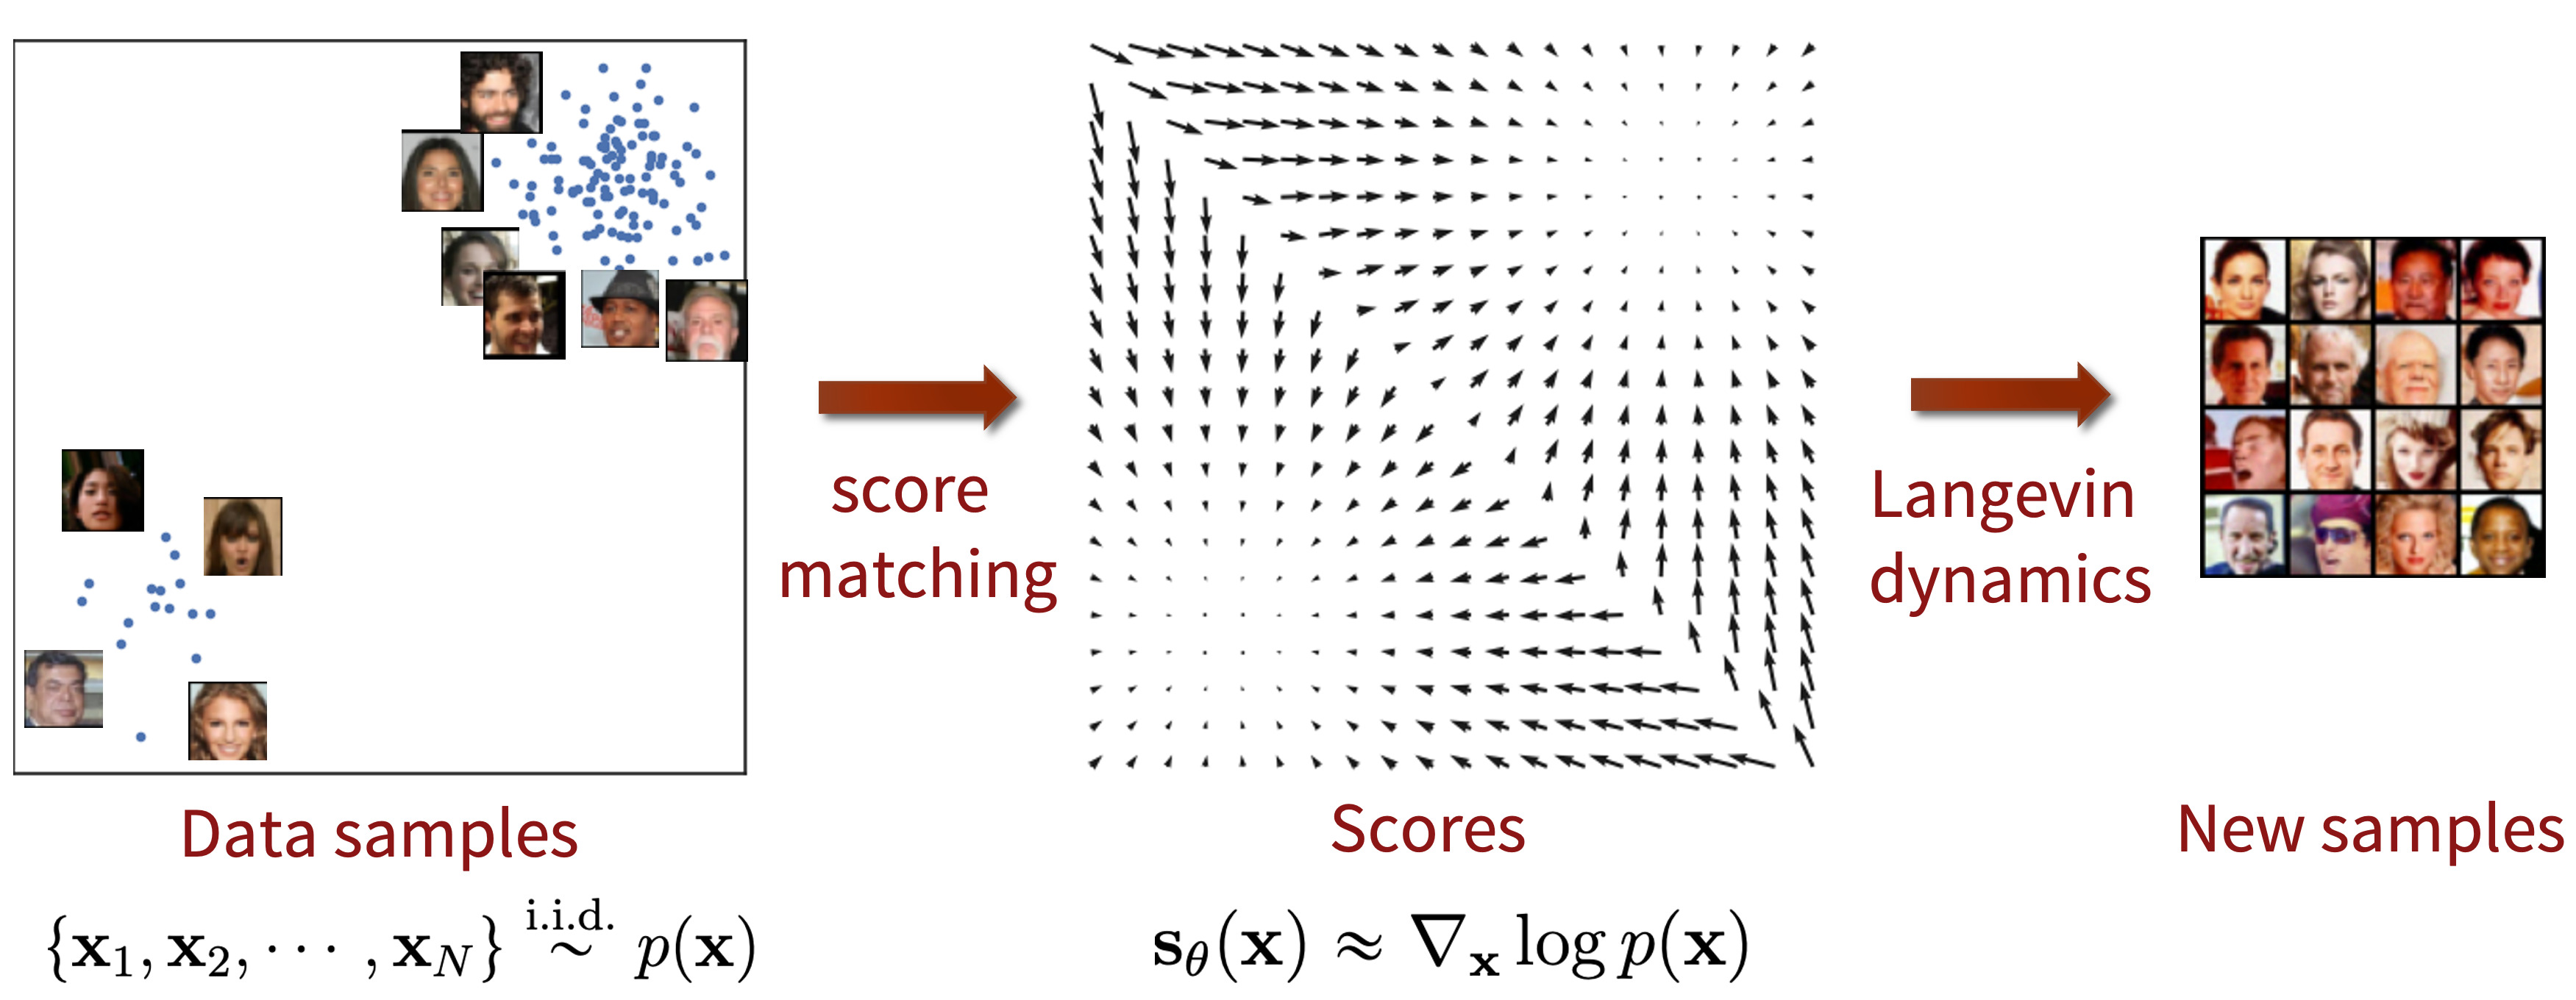
\includegraphics[width=0.9\linewidth]{figs/smld}
	\end{figure}
	\vspace{-0.3cm}
	\eqpause
	\begin{block}{Fisher Divergence}
		\vspace{-0.7cm}
		\begin{multline*}
			D_F(\pd, \pt) = \frac{1}{2}\bbE_{\pi}\big\| \nabla_{\bx}\log \pt(\bx) - \nabla_\bx \log \pd(\bx) \big\|^2_2 =\\
			= \frac{1}{2}\bbE_{\pi}\big\| \bs_{\btheta}(\bx) - \nabla_\bx \log \pd(\bx) \big\|^2_2 \rightarrow \min_{\btheta}
		\end{multline*}
		\vspace{-0.5cm}
	\end{block}
	\eqpause
	\textbf{Problem:} We don't know $\nabla_\bx \log \pd(\bx)$.
\end{frame}
%=======
\begin{frame}{Why Score Function is Better than Density?}
	\myfootnotewithlink{https://arxiv.org/abs/2510.21890}{Lai C. H. et al. The principles of diffusion models, 2025.}
	\begin{block}{Freedom from Normalization Constants}
		Many distributions are defined only up to an unnormalized density $\hat{p}(\bx)$:
		\vspace{-0.3cm}
		\[
			\nabla_{\bx} \log p(\bx) = \nabla_{\bx} \log \hat{p}(\bx) - \underbrace{\nabla_{\bx} \log Z}_{=0} = \nabla_{\bx} \log \hat{p}(\bx)
		\]
		\vspace{-0.3cm} \\
		The score function bypasses the intractable constant $Z$ entirely!
	\end{block}
	\eqpause
	\begin{block}{A Complete Representation}
		The score function fully characterizes the underlying distribution (up to a constant):
		\vspace{-0.2cm}
		\[
			\log p(\bx) = \log p(\bx_0) + \int_0^1 \bs(\bx_0 + t(\bx - \bx_0))^\top (\bx - \bx_0) dt
		\]
		\vspace{-0.5cm} \\
		Modeling the score is as expressive as modeling $p(\bx)$ itself, while often more tractable for generative modeling.
	\end{block}
\end{frame}
%=======
\subsection{Denoising Score Matching}
%=======
\begin{frame}{Denoising Score Matching}
	\myfootnotewithlink{http://www.iro.umontreal.ca/~vincentp/Publications/smdae_techreport.pdf}{Vincent P. A Connection Between Score Matching and Denoising Autoencoders, 2010}

	Let us perturb the original data $\bx \sim \pd(\bx)$ with Gaussian noise:
	\vspace{-0.3cm}
	\[
		\bx_{\sigma} = \bx + \sigma \cdot \bepsilon, \quad \bepsilon \sim \cN(0, \bI), \quad q(\bx_{\sigma} | \bx) = \cN(\bx, \sigma^2 \cdot \bI)
	\]
	\eqpause
	\vspace{-0.4cm}
	\[
		q(\bx_{\sigma}) = \int q(\bx_{\sigma} | \bx) \pd(\bx) d\bx.
	\]
	\eqpause
	\vspace{-0.5cm}
	\begin{block}{Assumption}
		The solution to
		\[
			\frac{1}{2} \bbE_{q(\bx_{\sigma})}\big\| \bs_{\btheta, \sigma}(\bx_{\sigma}) - \nabla_{\bx_{\sigma}} \log q(\bx_{\sigma}) \big\|^2_2 \rightarrow \min_{\btheta}
		\]
		\vspace{-0.3cm} \\
		satisfies $\bs_{\btheta, \sigma}(\bx_{\sigma}) \approx \bs_{\btheta, 0}(\bx_0) = \bs_{\btheta}(\bx)$ if $\sigma$ is sufficiently small.
	\end{block}
	\eqpause
	\begin{itemize}
		\item The score function of the noised data nearly matches the score function of the original data.
		\item The score function $\bs_{\btheta, \sigma}(\bx_{\sigma})$ is parameterized by $\sigma$.
		\item \textbf{Note:} We don't know $q(\bx_{\sigma})$, just as we don't know $\pd(\bx)$.
	\end{itemize}
\end{frame}
%=======
\begin{frame}{Denoising Score Matching}
	\myfootnotewithlink{http://www.iro.umontreal.ca/~vincentp/Publications/smdae_techreport.pdf}{Vincent P. A Connection Between Score Matching and Denoising Autoencoders, 2010}
	\begin{block}{Theorem}
		Under mild regularity conditions, the following holds:
		\vspace{-0.3cm}
		\begin{multline*}
			\bbE_{q(\bx_{\sigma})}\big\| \bs_{\btheta, \sigma}(\bx_{\sigma}) - \nabla_{\bx_{\sigma}} \log q(\bx_{\sigma}) \big\|^2_2 = \\
		= \bbE_{\pd(\bx)} \bbE_{q(\bx_{\sigma} | \bx)}\big\| \bs_{\btheta, \sigma}(\bx_{\sigma}) - \nabla_{\bx_{\sigma}} \log q(\bx_{\sigma} | \bx) \big\|^2_2 + \text{const}(\btheta)
		\end{multline*}
		\vspace{-0.5cm}
	\end{block}
	\eqpause
	\begin{block}{Gradient of the Noise Kernel}
		\vspace{-0.3cm}
		\[
			\bx_{\sigma} = \bx + \sigma \cdot \bepsilon, \quad q(\bx_{\sigma} | \bx) = \cN(\bx, \sigma^2 \cdot \bI)
		\]
		\eqpause
		\vspace{-0.3cm}
		\[
			\nabla_{\bx_{\sigma}} \log q(\bx_{\sigma} | \bx) = - \frac{\bx_{\sigma} - \bx}{\sigma^2}  = - \frac{\bepsilon}{\sigma}
		\]
		\eqpause
		\vspace{-0.5cm}
	\end{block}
	\begin{itemize}
		\item The right-hand side doesn't require computing $\nabla_{\bx_{\sigma}} \log q(\bx_{\sigma})$ or even $\nabla_{\bx_{\sigma}} \log \pd(\bx_{\sigma})$.
		\item $\bs_{\btheta, \sigma}(\bx_{\sigma})$ is trained to \textbf{denoise} the noised samples $\bx_{\sigma}$.
	\end{itemize}
\end{frame}
%=======
\begin{frame}{Denoising Score Matching}
	\myfootnotewithlink{https://yang-song.github.io/blog/2021/score/}{Song Y. Generative Modeling by Estimating Gradients of the Data Distribution, blog post, 2021}
	Initial objective:
	\vspace{-0.2cm}
	\[
		\bbE_{\pd(\bx)}\big\| \bs_{\btheta}(\bx) - \nabla_\bx \log \pd(\bx) \big\|^2_2 \rightarrow \min_{\btheta}
	\]
	\eqpause
	\vspace{-0.5cm} \\
	Noised objective:
	\vspace{-0.2cm}
	\[
		\bbE_{q(\bx_{\sigma})}\big\| \bs_{\btheta, \sigma}(\bx_\sigma) - \nabla_\bx \log q(\bx_{\sigma}) \big\|^2_2 \rightarrow \min_{\btheta}
	\]
	\eqpause
	\vspace{-0.5cm} \\
	This is equivalent to a denoising task:
	\vspace{-0.2cm}
	\[
		\bbE_{\pd(\bx)} \bbE_{q(\bx_{\sigma} | \bx)}\big\| \bs_{\btheta, \sigma}(\bx_{\sigma}) - \nabla_{\bx_{\sigma}} \log q(\bx_{\sigma} | \bx) \big\|^2_2 \rightarrow \min_{\btheta}
	\]
	\eqpause
	\vspace{-0.3cm}
	\[
		\bbE_{\pd(\bx)} \bbE_{\cN(0, \bI)}\left\| \bs_{\btheta, \sigma}(\bx + \sigma \cdot \bepsilon) + \frac{\bepsilon}{\sigma} \right\|^2_2 \rightarrow \min_{\btheta}
	\]
	\vspace{-0.5cm}
	\begin{block}{Langevin Dynamics}
		\vspace{-0.3cm}
		\[
			\bx_{l + 1} = \bx_l + \frac{\eta}{2} \cdot \bs_{\btheta, \sigma}(\bx_l) + \sqrt{\eta} \cdot \bepsilon_l, \quad \bepsilon_l \sim \cN(0, \bI).
		\]
		\vspace{-0.7cm}
	\end{block}
\end{frame}
%=======
\begin{frame}{Denoising Score Matching}
    \myfootnotewithlink{http://www.iro.umontreal.ca/~vincentp/Publications/smdae_techreport.pdf}{Vincent P. A Connection Between Score Matching and Denoising Autoencoders, 2010}
	\begin{block}{Theorem}
	\vspace{-0.5cm}
	\begin{multline*}
		\bbE_{q(\bx_{\sigma})}\underbrace{\left\| \bs_{\btheta, \sigma}(\bx_{\sigma}) - \nabla_{\bx_{\sigma}} \log q(\bx_{\sigma}) \right\|_2^2}_{h(\bx_{\sigma})} = \\
		= \bbE_{\pd(\bx)} \bbE_{q(\bx_{\sigma} | \bx)}\left\| \bs_{\btheta, \sigma}(\bx_{\sigma}) - \nabla_{\bx_{\sigma}} \log q(\bx_{\sigma} | \bx) \right\|_2^2 + \text{const}(\btheta)
	\end{multline*}
	\vspace{-0.5cm}
	\end{block}
    \eqpause
	\begin{block}{Proof}
		\vspace{-0.7cm}
		\begin{multline*}
			\bbE_{q(\bx_{\sigma})} h(\bx_{\sigma}) = \int {\color{violet}q(\bx_{\sigma})} h(\bx_{\sigma}) d\bx_{\sigma} 
			\nextonslide{= \\ = \int \left({\color{violet}\int q(\bx_{\sigma} | \bx) \pd(\bx) d\bx}\right) h(\bx_{\sigma}) d\bx_{\sigma} =  \bbE_{\pd(\bx)} \bbE_{q(\bx_{\sigma} | \bx)}  h(\bx_{\sigma})}
		\end{multline*}
        \eqpause
		\vspace{-0.7cm}
		{\small
		\begin{multline*}
			\bbE_{q(\bx_{\sigma})}\left\| \bs_{\btheta, \sigma}(\bx_{\sigma}) - \nabla_{\bx_{\sigma}} \log q(\bx_{\sigma}) \right\|_2^2 = \\ 
			\nextonslide{= \bbE_{q(\bx_{\sigma})} \Bigl[\| \bs_{\btheta, \sigma}(\bx_{\sigma}) \|^2 + \underbrace{\| \nabla_{\bx_{\sigma}} \log q(\bx_{\sigma}) \|_2^2}_{\text{const}(\btheta)} - 2 {\color{teal}\bs_{\btheta, \sigma}^\top(\bx_{\sigma}) \nabla_{\bx_{\sigma}} \log q(\bx_{\sigma})} \Bigr]}
		\end{multline*}
		}
	\end{block}
\end{frame}
%=======
\begin{frame}{Denoising Score Matching}
    \myfootnotewithlink{http://www.iro.umontreal.ca/~vincentp/Publications/smdae_techreport.pdf}{Vincent P. A Connection Between Score Matching and Denoising Autoencoders, 2010}
	\begin{block}{Theorem}
		\vspace{-0.5cm}
		\begin{multline*}
			\bbE_{q(\bx_{\sigma})}\left\| \bs_{\btheta, \sigma}(\bx_{\sigma}) - \nabla_{\bx_{\sigma}} \log q(\bx_{\sigma}) \right\|_2^2 = \\
			= \bbE_{\pd(\bx)} \bbE_{q(\bx_{\sigma} | \bx)}\left\| \bs_{\btheta, \sigma}(\bx_{\sigma}) - \nabla_{\bx_{\sigma}} \log q(\bx_{\sigma} | \bx) \right\|_2^2 + \text{const}(\btheta)
		\end{multline*}
		\vspace{-0.5cm}
	\end{block}
	\begin{block}{Proof (Continued)}
		\vspace{-0.7cm}
		{\small
		\begin{multline*}
			\bbE_{q(\bx_{\sigma})} \left[{\color{teal}\bs_{\btheta, \sigma}^\top(\bx_{\sigma}) \nabla_{\bx_{\sigma}} \log q(\bx_{\sigma})} \right] 
			\nextonslide{= \int q(\bx_{\sigma}) \left[\bs_{\btheta, \sigma}^\top(\bx_{\sigma}) \frac{\nabla_{\bx_{\sigma}} {\color{violet}q(\bx_{\sigma})}}{q(\bx_{\sigma})} \right] d\bx_{\sigma}}
			\nextonslide{= \\ = \int \left[\bs_{\btheta, \sigma}^\top(\bx_{\sigma}) \nabla_{\bx_{\sigma}}\left({\color{violet}\int q(\bx_{\sigma} | \bx) \pd(\bx) d\bx}\right) \right] d\bx_{\sigma}}
			\nextonslide{ = \\ =  \int \int \pd(\bx) \left[\bs_{\btheta, \sigma}^\top(\bx_{\sigma}) {\color{olive}\nabla_{\bx_{\sigma}}q(\bx_{\sigma} | \bx)} \right] d\bx_{\sigma} d\bx}
			\nextonslide{ = \\ = \int \int \pd(\bx) {\color{olive} q(\bx_{\sigma} | \bx)} \left[\bs_{\btheta, \sigma}^\top(\bx_{\sigma}) {\color{olive}\nabla_{\bx_{\sigma}} \log q(\bx_{\sigma} | \bx)} \right] d\bx_{\sigma} d\bx}
			\nextonslide{ = \\ = \bbE_{\pd(\bx)} \bbE_{q(\bx_{\sigma} | \bx)} \left[{\color{teal}\bs_{\btheta, \sigma}^\top(\bx_{\sigma}) \nabla_{\bx_{\sigma}} \log q(\bx_{\sigma} | \bx)} \right]}
		\end{multline*}
		}
	\end{block}
\end{frame}
%=======
\begin{frame}{Denoising Score Matching}
    \myfootnotewithlink{http://www.iro.umontreal.ca/~vincentp/Publications/smdae_techreport.pdf}{Vincent P. A Connection Between Score Matching and Denoising Autoencoders, 2010}
	\vspace{-0.3cm}
	\begin{block}{Theorem}
		\vspace{-0.7cm}
		\begin{multline*}
			\bbE_{q(\bx_{\sigma})}\underbrace{\left\| \bs_{\btheta, \sigma}(\bx_{\sigma}) - \nabla_{\bx_{\sigma}} \log q(\bx_{\sigma}) \right\|_2^2}_{h(\bx_{\sigma})} = \\
			= \bbE_{\pd(\bx)} \bbE_{q(\bx_{\sigma} | \bx)}\left\| \bs_{\btheta, \sigma}(\bx_{\sigma}) - \nabla_{\bx_{\sigma}} \log q(\bx_{\sigma} | \bx) \right\|_2^2 + \text{const}(\btheta)
		\end{multline*}
		\vspace{-0.9cm}
	\end{block}
	\begin{block}{Proof (Continued)}
		\vspace{-0.3cm}
		\[
			\bbE_{q(\bx_{\sigma})} h(\bx_{\sigma})=  \bbE_{\pd(\bx)} \bbE_{q(\bx_{\sigma} | \bx)}  h(\bx_{\sigma})
		\]
        \eqpause
		{\small
		\[
			\bbE_{q(\bx_{\sigma})} \left[\bs_{\btheta, \sigma}^\top(\bx_{\sigma}) \nabla_{\bx_{\sigma}} \log q(\bx_{\sigma}) \right] = \bbE_{\pd(\bx)} \bbE_{q(\bx_{\sigma} | \bx)} \left[\bs_{\btheta, \sigma}^\top(\bx_{\sigma}) \nabla_{\bx_{\sigma}} \log q(\bx_{\sigma} | \bx) \right]
		\]
        \eqpause
		\vspace{-0.5cm}
		\begin{multline*}
			\bbE_{q(\bx_{\sigma})}\left\| \bs_{\btheta, \sigma}(\bx_{\sigma}) - \nabla_{\bx_{\sigma}} \log q(\bx_{\sigma}) \right\|_2^2 = \\ 
			= {\color{olive}\bbE_{\pd(\bx)} \bbE_{q(\bx_{\sigma} | \bx)}}\left[\| \bs_{\btheta, \sigma}(\bx_{\sigma}) \|^2 - 2 \bs_{\btheta, \sigma}^\top(\bx_{\sigma}) {\color{teal}\nabla_{\bx_{\sigma}} \log q(\bx_{\sigma} | \bx)} \right] + \text{const}(\btheta)
			\nextonslide{= \\ = {\color{olive}\bbE_{\pd(\bx)} \bbE_{q(\bx_{\sigma} | \bx)}} \left\|\bs_{\btheta, \sigma}(\bx_{\sigma}) - {\color{teal}\nabla_{\bx_{\sigma}} \log q(\bx_{\sigma} | \bx)} \right\|_2^2 + \text{const}(\btheta)}
		\end{multline*}
		}
		\vspace{-0.8cm}
	\end{block}
\end{frame}
%=======
\begin{frame}{Denoising Score Matching}
	\myfootnotewithlink{http://www.iro.umontreal.ca/~vincentp/Publications/smdae_techreport.pdf}{Vincent P. A Connection Between Score Matching and Denoising Autoencoders, 2010}
	\begin{block}{Denoising Score Matching Objective}
		\vspace{-0.3cm}
		\[
			\bbE_{\pd(\bx)} \bbE_{q(\bx_{\sigma} | \bx)}\left\| \bs_{\btheta, \sigma}(\bx_{\sigma}) - \nabla_{\bx_{\sigma}} \log q(\bx_{\sigma} | \bx) \right\|_2^2 \rightarrow \min_{\btheta}
		\]
		\vspace{-0.5cm}
	\end{block}
	\eqpause
	The optimal MSE predictor is the posterior mean of the regression target:
	\[
		\bs_{\btheta^*, \sigma}(\bx_\sigma) = \bbE_{q(\bx | \bx_\sigma)} \left[\nabla_{\bx_\sigma} \log q(\bx_\sigma | \bx) \right]
	\]
	\eqpause
	\vspace{-0.5cm}
	\begin{block}{Marginal Score via Conditional Scores}
		\vspace{-0.5cm}
		\begin{multline*}
			\nabla_{\bx_\sigma} \log q(\bx_\sigma) = \frac{\nabla_{\bx_\sigma} {\color{violet}\int q(\bx_\sigma | \bx) \pd(\bx) d\bx}}{q(\bx_\sigma)}
			\nextonslide{= \\ = \int \nabla_{\bx_\sigma} \log q(\bx_\sigma | \bx) \cdot {\color{olive}\frac{q(\bx_\sigma | \bx) \pd(\bx)}{q(\bx_\sigma)}} d\bx}
			\nextonslide{= \bbE_{\color{olive}q(\bx | \bx_\sigma)} \left[\nabla_{\bx_\sigma} \log q(\bx_\sigma | \bx) \right]}
		\end{multline*}
		\vspace{-0.5cm}
	\end{block}
	\eqpause
	\textbf{Therefore:} $\bs_{\btheta^*, \sigma}(\bx_\sigma) = \nabla_{\bx_\sigma} \log q(\bx_\sigma)$ -- the optimal model learns the true \textbf{marginal} score!
\end{frame}
%=======
\begin{frame}{Denoising Score Matching}
    \myfootnotewithlink{https://yang-song.github.io/blog/2021/score/}{Song Y. Generative Modeling by Estimating Gradients of the Data Distribution, blog post, 2021}
	Original objective:
	\vspace{-0.2cm}
	\[
		\bbE_{\pd(\bx)}\left\| \bs_{\btheta}(\bx) - \nabla_\bx \log \pd(\bx) \right\|_2^2 \rightarrow \min_{\btheta}
	\]
    \eqpause
	\vspace{-0.5cm} \\
	Noisy objective:
	\vspace{-0.2cm}
	\[
		\bbE_{q(\bx_{\sigma})}\left\| \bs_{\btheta, \sigma}(\bx_\sigma) - \nabla_\bx \log q(\bx_{\sigma}) \right\|_2^2 \rightarrow \min_{\btheta}
	\]
    \eqpause
	\vspace{-0.5cm} \\
	This is equivalent to a denoising task:
	\vspace{-0.2cm}
	\[
		\bbE_{\pd(\bx)} \bbE_{q(\bx_{\sigma} | \bx)}\left\| \bs_{\btheta, \sigma}(\bx_{\sigma}) - \nabla_{\bx_{\sigma}} \log q(\bx_{\sigma} | \bx) \right\|_2^2 \rightarrow \min_{\btheta}
	\]
    \eqpause
	\vspace{-0.3cm}
	\[
		\bbE_{\pd(\bx)} \bbE_{\cN(0, \bI)}\left\| \bs_{\btheta, \sigma}(\bx + \sigma \bepsilon) + \frac{\bepsilon}{\sigma} \right\|_2^2 \rightarrow \min_{\btheta}
	\]
    \eqpause
	\vspace{-0.5cm}
	\begin{block}{Langevin Dynamics}
		\vspace{-0.3cm}
		\[
			\bx_{l + 1} = \bx_l + \frac{\eta}{2} \cdot \bs_{\btheta, \sigma}(\bx_l) + \sqrt{\eta} \cdot \bepsilon_l, \quad \bepsilon_l \sim \cN(0, \bI)
		\]
		\vspace{-0.7cm}
	\end{block}
\end{frame}
%=======
\subsection{Noise-Conditioned Score Network (NCSN)}
%=======
\begin{frame}{Denoising Score Matching}
    \myfootnotewithlink{https://yang-song.github.io/blog/2021/score/}{Song Y. Generative Modeling by Estimating Gradients of the Data Distribution, blog post, 2021}
	\vspace{-0.5cm}
	\[
		\bbE_{\pd(\bx)} \bbE_{\cN(0, \bI)}\left\| \bs_{\btheta, \sigma}(\bx + \sigma \bepsilon) + \frac{\bepsilon}{\sigma} \right\|_2^2 \rightarrow \min_{\btheta}
	\]
	\begin{minipage}{0.5\linewidth}
		\[
			\bx_{l + 1} = \bx_l + \frac{\eta}{2} \cdot \bs_{\btheta, \sigma}(\bx_l) + \sqrt{\eta} \cdot \bepsilon_l
		\]
		\vspace{-0.3cm}
		\begin{itemize}
			\item For \textbf{small} $\sigma$, $\bs_{\btheta, \sigma}(\bx)$ becomes inaccurate and Langevin dynamics fails to traverse modes
			\item For \textbf{large} $\sigma$, robustness in low-density regions is achieved, but the model learns a distribution that is overly corrupted
		\end{itemize}
	\end{minipage}%
	\begin{minipage}{0.5\linewidth}
		\begin{figure}
			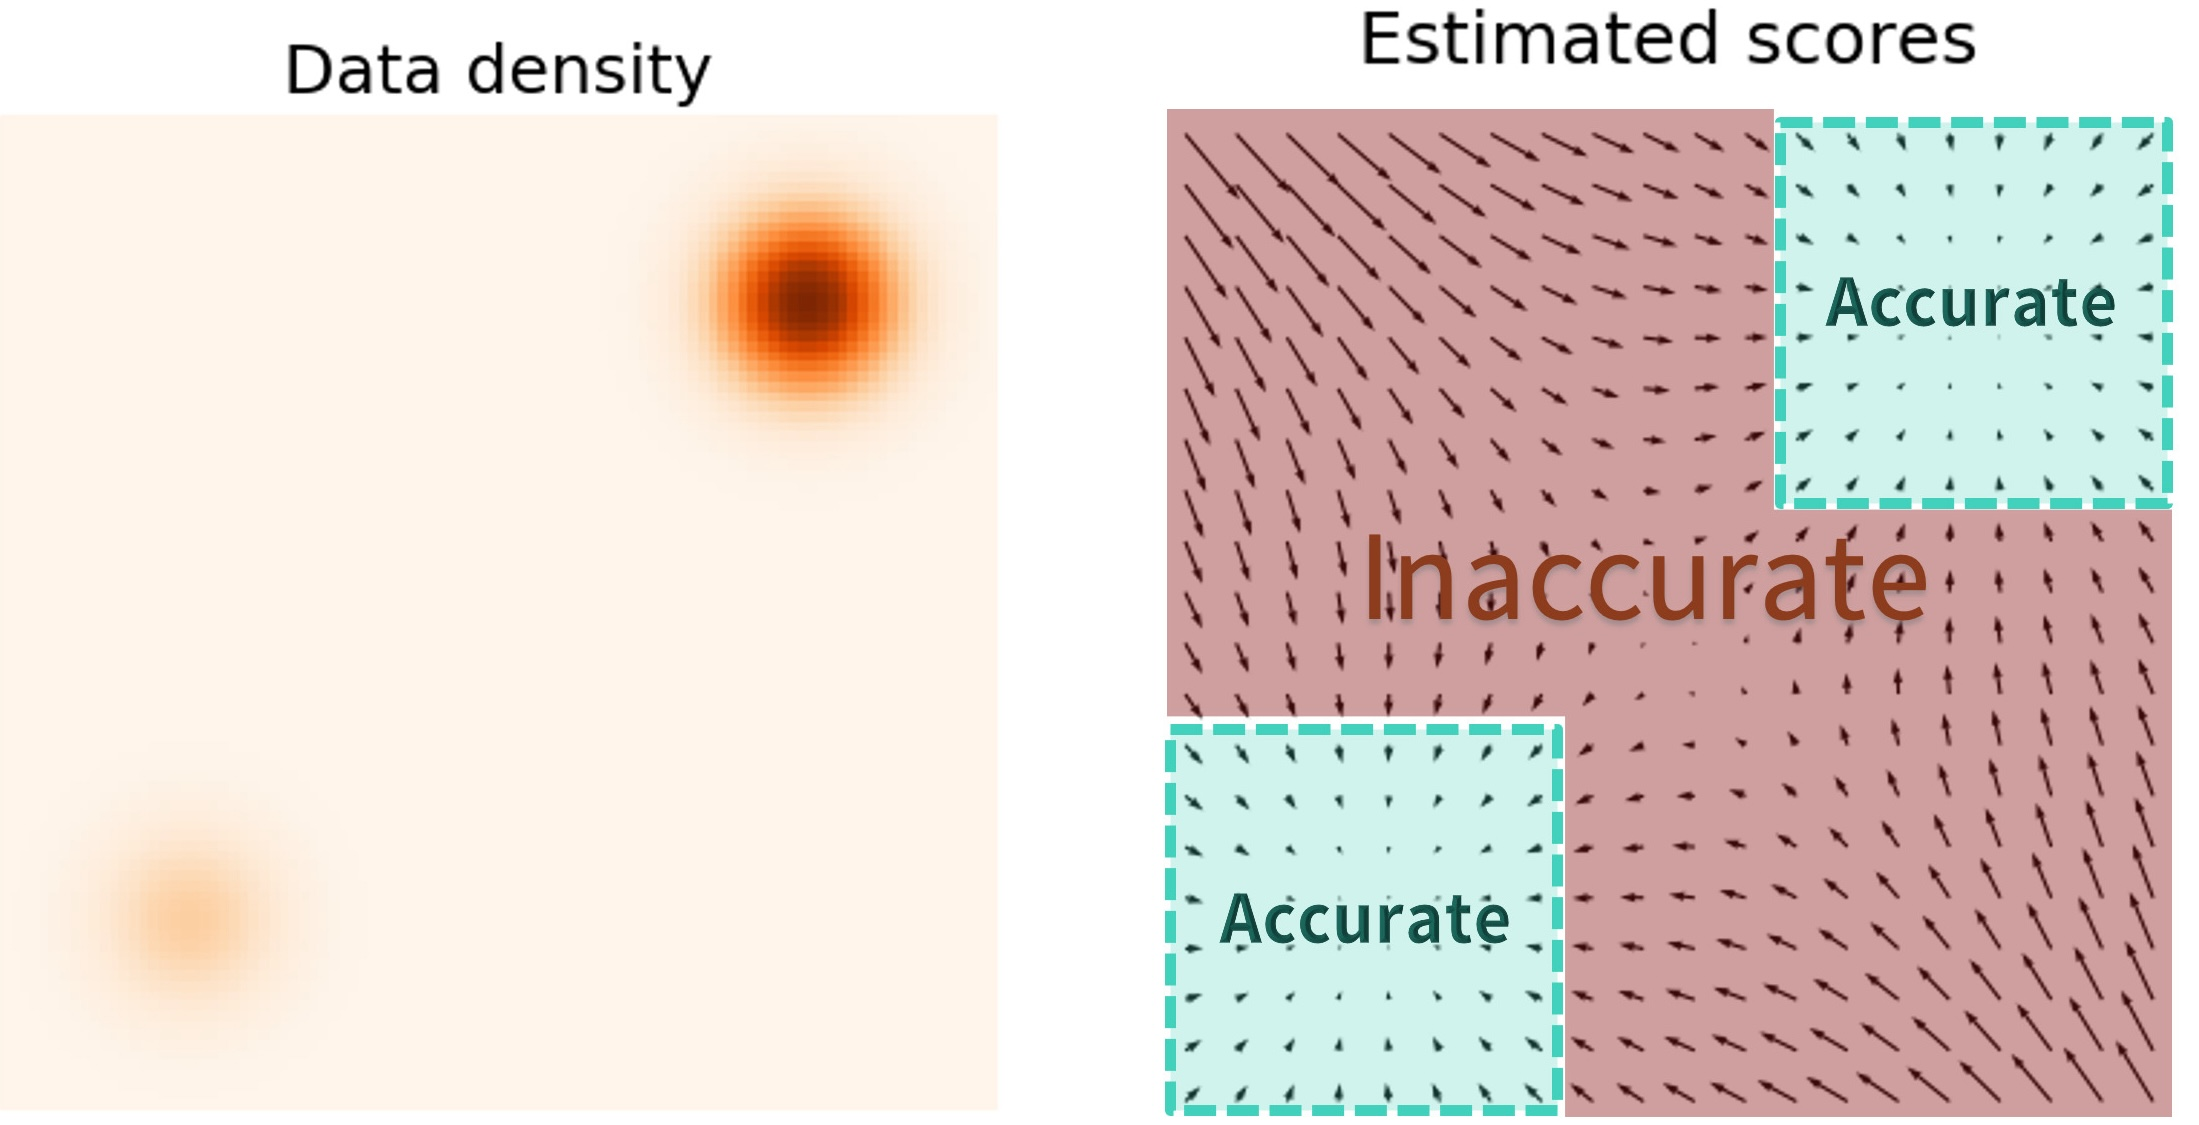
\includegraphics[width=\linewidth]{figs/pitfalls}
		\end{figure}
		\vspace{-0.3cm}
		\begin{figure}
			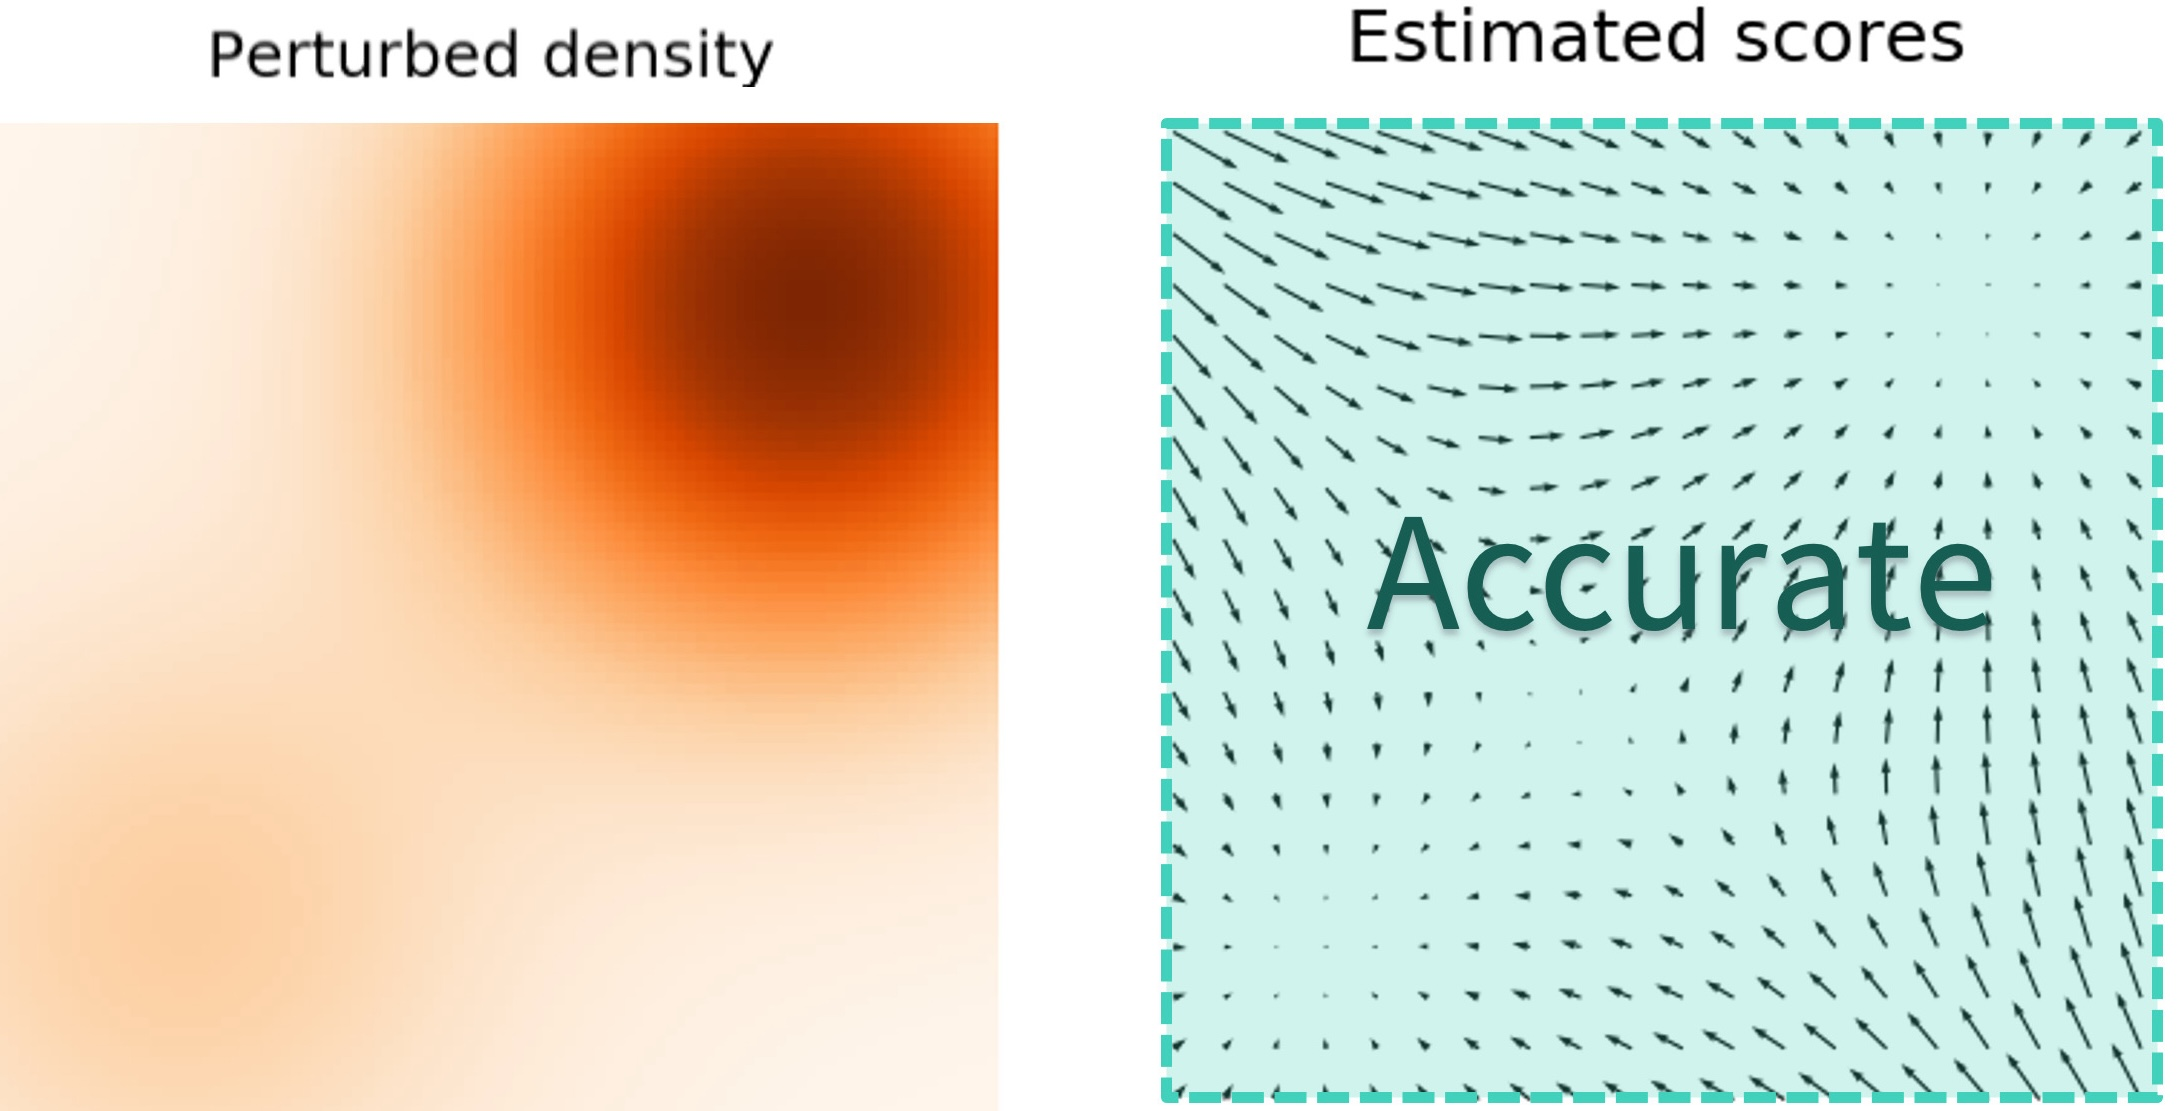
\includegraphics[width=\linewidth]{figs/single_noise}
		\end{figure}
	\end{minipage}
\end{frame}
%=======
\begin{frame}{Noise-Conditioned Score Network (NCSN)}
    \myfootnotewithlink{https://arxiv.org/abs/1907.05600}{Song Y. et al. Generative Modeling by Estimating Gradients of the Data Distribution, 2019}
	\begin{itemize}
		\item Specify a sequence of noise levels: $\sigma_1 < \sigma_2 < \dots < \sigma_T$
		\item Perturb each data point with different noise levels: $\bx_t = \bx + \sigma_t \bepsilon$, so $\bx_t \sim q(\bx_t)$
		\item Choose $\sigma_1, \sigma_T$ such that:
		\[
			q(\bx_1) \approx \pd(\bx), \;\; q(\bx_T) \approx \cN(0, \sigma_T^2 \bI)
		\]
	\end{itemize}
    \eqpause
	\vspace{-0.3cm}
	\begin{figure}
		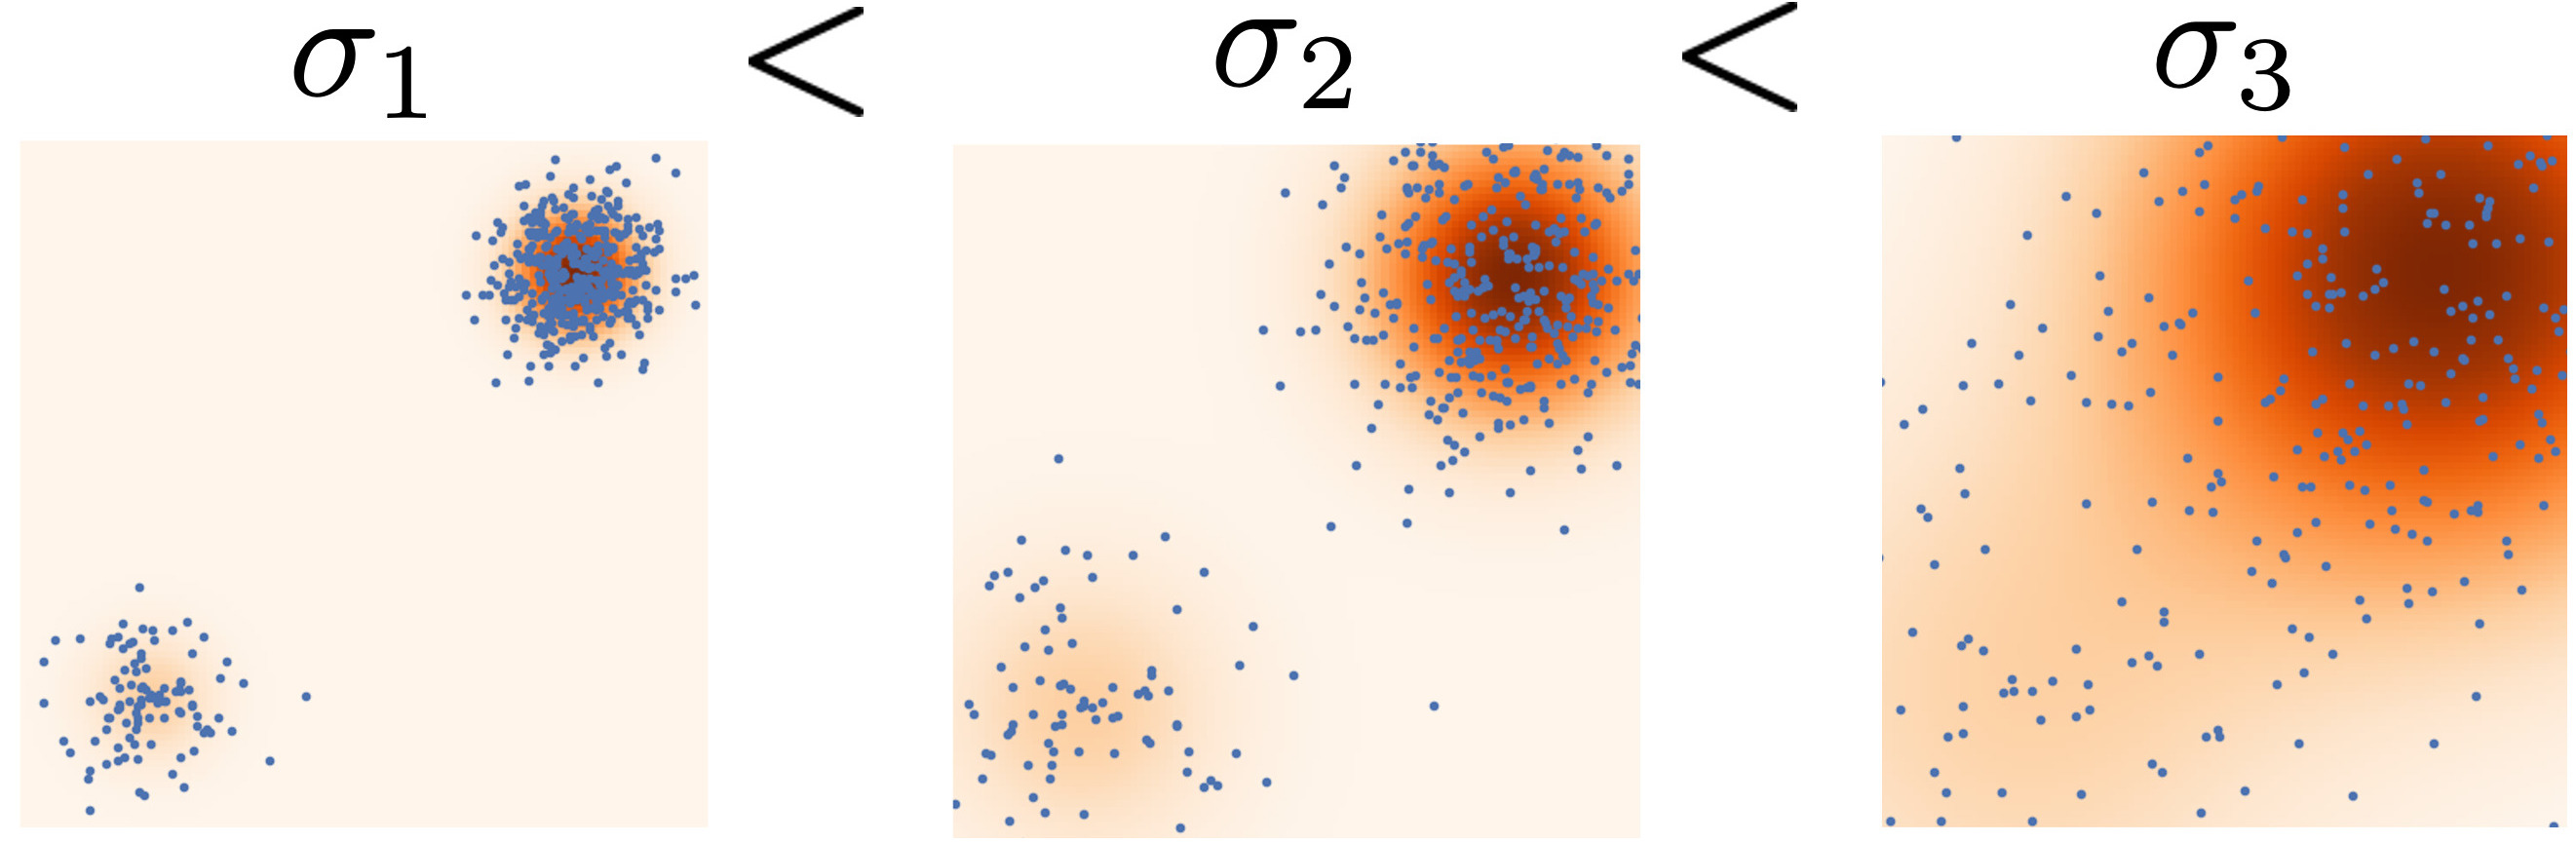
\includegraphics[width=0.6\linewidth]{figs/multi_scale}
	\end{figure}
	\begin{figure}
		
\includegraphics[width=\linewidth]{figs/duoduo}
	\end{figure}
\end{frame}
%=======
\begin{frame}{Noise-Conditioned Score Network (NCSN)}
    \myfootnotewithlink{https://arxiv.org/abs/1907.05600}{Song Y. et al. Generative Modeling by Estimating Gradients of the Data Distribution, 2019}
	Train the denoising score function $\bs_{\btheta, \sigma_t}(\bx_t)$ for each noise level $\sigma_t$ using a unified weighted objective:
	\vspace{-0.2cm}
	\[
		\sum_{t=1}^T {\color{violet}\sigma_t^2} \bbE_{\pd(\bx)} \bbE_{q(\bx_t | \bx)}\left\| \bs_{\btheta, \sigma_t}(\bx_t) - \nabla_{\bx_t} \log q(\bx_t | \bx) \right\|_2^2 \rightarrow \min_{\btheta}
	\]
    \eqpause
	Here, $\nabla_{\bx_t} \log q(\bx_t | \bx) = - \frac{\bx_t - \bx}{\sigma_t^2} = - \frac{\bepsilon}{\sigma_t}$
    \eqpause
	\begin{block}{Training}
		\begin{enumerate}
			\item Sample $\bx_0 \sim \pd(\bx)$.
			\item Sample $t \sim U\{1, T\}$, $\bepsilon \sim \cN(0, \bI)$.
			\item Compute noisy image $\bx_t = \bx_0 + \sigma_t \bepsilon$.
			\item Compute loss $ \cL = \sigma_t^2 \left\| \bs_{\btheta, \sigma_t}(\bx_t) + \frac{\bepsilon}{\sigma_t} \right\|^2 $.
		\end{enumerate}
		\vspace{-0.3cm}
	\end{block}
    \eqpause
	How do we sample from such a model?
\end{frame}
%=======
\begin{frame}{Noise-Conditioned Score Network (NCSN)}
    \myfootnotewithlink{https://arxiv.org/abs/2006.09011}{Song Y. et al. Improved Techniques for Training Score-Based Generative Models, 2020}
	\begin{block}{Sampling (Annealed Langevin Dynamics)}
		\begin{enumerate}
			\item Sample $\bx_0 \sim \cN(0, \sigma_T^2 \bI) \approx q(\bx_T)$.
			\item At each noise level, apply $L$ steps of Langevin dynamics:
			\vspace{-0.2cm}
			\[
				\bx_l = \bx_{l-1} + \frac{\eta_t}{2} \bs_{\btheta, \sigma_t}(\bx_{l-1}) + \sqrt{\eta_t} \bepsilon_l.
			\]
			\vspace{-0.5cm}
			\item Update $\bx_0 := \bx_L$ and reduce to the next lower $\sigma_t$.
		\end{enumerate}
	\end{block}
    \eqpause
	\begin{figure}
		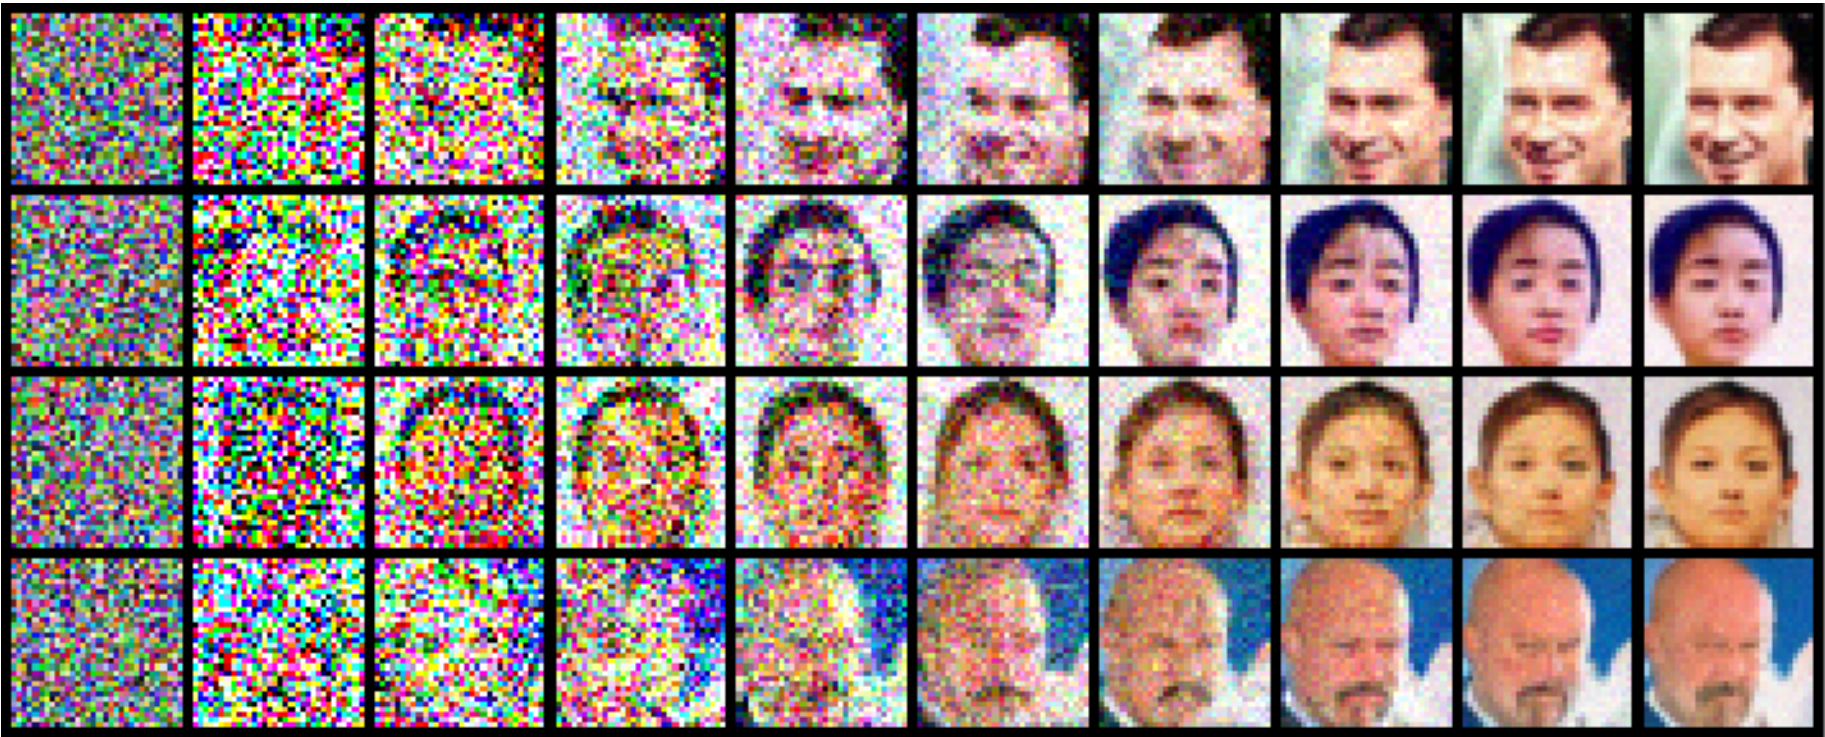
\includegraphics[width=0.9\linewidth]{figs/ald}
	\end{figure}
\end{frame}
%=======
\begin{frame}{Summary}
	\begin{itemize}
		\item Langevin dynamics enable sampling from generative models using gradients of the log-likelihood.
		\vfill
		\item Score matching proposes minimizing Fisher divergence to estimate the score function.
		\vfill
		\item Denoising score matching minimizes the Fisher divergence on corrupted samples, making the divergence estimable via sampling.
		\vfill 
		\item The Noise-Conditioned Score Network leverages a range of noise levels and annealed Langevin dynamics to learn the score function and enable sampling	
	\end{itemize}
\end{frame}
\end{document}